\documentclass[paper=a4, open=any, numbers=noenddot]{scrbook}

\usepackage[hang]{caption}
\usepackage{microtype}
\usepackage[intlimits]{mathtools}
\usepackage{amsfonts, amssymb, longtable, array, xltabular, scrlayer-scrpage}
\usepackage[per-mode=fraction, locale=DE, detect-all=true]{siunitx}
\usepackage{unicode-math, icomma}
\usepackage{fontspec}
\usepackage{polyglossia}
\setdefaultlanguage[spelling=new]{german}
\usepackage[autostyle]{csquotes}
\usepackage[margin=20mm, bottom=15mm, includefoot]{geometry}
\usepackage{graphicx, xcolor}
\usepackage{datetime, float}
%\usepackage[section]{placeins}
\usepackage[unicode=true, colorlinks=false, breaklinks=true, pdfborder={0 0 0}]{hyperref}
\usepackage{bookmark}

\hypersetup{pdfinfo={
		Title    = {FUOCO STEP - Aufbau- und Bedienungsanleitung},
		Subject  = {Handbuch},
		Author   = {Felix Pflaum}
}}


\makeatletter
\@addtoreset{chapter}{part}
\makeatother  

\newcommand{\origttfamily}{}
\let\origttfamily=\ttfamily
\renewcommand{\ttfamily}{\origttfamily \hyphenchar\font=`\-}
\setmainfont{Tex Gyre Termes}
\setmathfont{Tex Gyre Termes Math}
\setmathfont{TeX Gyre Termes}[range=\mathup/{latin,Latin,num}]
\setsansfont{Latin Modern Sans}[Scale=MatchLowercase]
\setmonofont{LMMonoLt10-Bold}[Scale=MatchLowercase]
\AtBeginDocument{%
	\let\umathpi\pi%ersatzbefehl für kursives pi
	\renewcommand\pi{\symup\umathpi}%alle \pi per default aufrecht
}
\newfontfamily\Commons{Commons}
\newfontfamily\Gost{Gost}
\defaultfontfeatures{Ligatures=TeX}

\renewcommand{\dateseparator}{.}

% Einstellungen für den Zeilenumbruch von URLs
\def\UrlBreaks{\do\=\do\.\do\?\do\&\do\a\do\b\do\c\do\d\do\e\do\f\do\g\do\h\do\i\do\j\do\k\do\l\do\m\do\n\do\o\do\p\do\q\do\r\do\s\do\t\do\u\do\v\do\w\do\x\do\y\do\z\do\A\do\B\do\C\do\D\do\E\do\F\do\G\do\H\do\I\do\J\do\K\do\L\do\M\do\N\do\O\do\P\do\Q\do\R\do\S\do\T\do\U\do\V\do\W\do\X\do\Y\do\Z\do\1\do\2\do\3\do\4\do\5\do\6\do\7\do\8\do\9\do\0}
\Urlmuskip = 0mu plus 1mu


\title{Aufbauanleitung FUOCO STEP}
\author{Felix Pflaum}
\date{31.05.2018}

\begin{document}
\begin{titlepage}
	\vspace*{\fill}
	\begin{center}
		\includegraphics[width=.9\textwidth]{Bilder/logo}
	\end{center}
	\vfill
	\begin{center}{\fontsize{40pt}{40pt} \Commons{Aufbau- und Bedienungsanleitung}} \vspace{5mm} \\
		{\fontsize{24pt}{24pt} \Gost{Felix Pflaum}} \vspace{3mm} \\
		{\fontsize{20pt}{20pt} \Gost{f.pflaum@gmail.com}} \vspace{5mm} \\
		{\fontsize{16pt}{16pt} \Gost{Stand: \ddmmyyyydate\today}}
	\end{center}
	\vfill
\end{titlepage}
\tableofcontents
\part{Aufbauanleitung}
	\chapter{Vorbereitung}
		FUOCO STEP besteht aus zwei Platinen (=PCBs), der Basis (kleine Platine) und dem Panel (große Platine), zum Lieferumfang des Bausatzes gehören neben den Platinen und ihren Lötteilen, die in den Tabellen~\ref{tab:bauteilepanel} und~\ref{tab:bauteilebasis} in den jeweiligen Unterkapiteln aufgeführt wurden:
		\begin{itemize}
			\item
			      Koffer Seahorse SE-120
			\item
			      Blei-Gel-Akku \SI{12}{\volt}/\SI{1,2}{\ampere\hour}
			\item
			      Hauptschalter mit blauer LED
			\item
			      Spannungsanzeige
			\item
			      Micro-USB-Anschluss für Gehäusemontage
			\item
			      Schlüsselschalter
			\item
			      Druckschalter für Durchgangstest
			\item
			      Drehschalter mit elf Widerständen und drei Kabeln (rot, gelb, schwarz)
			\item
			      Crimpbuchse mit drei Kabeln (rot, weiß, grau)
			\item
			      Crimpbuchse mit acht Kabeln (blau, schwarz, rot, schwarz, violett, violett, gelb, gelb)
			\item
			      Je ein rotes und ein schwarzes Kabel mit Kabelschuh
			\item
			      Je ein rotes und ein schwarzes Kabel ohne Kabelschuh
			\item
			      Ein Paar Deans-Steckverbinder (Buchse für Anschluss an Batterie, Stecker an PCB) mit Lötanschlüssen
			\item
			      Isolationsabdeckung für Lötkontakte auf der Paneloberseite
			\item
			      Vier Distanzhülsen der Länge \SI{11}{\milli\metre} als Abstandshalter zwischen Basis und Panel
			\item
			      Vier Gewindeschrauben M3x16 mit Muttern zur Verschraubung der beiden Platinen
			\item
			      Zwei Gewindeschrauben M3x6 mit Muttern zur Befestigung der Lötstellenabdeckung am Panel
			\item
			      Zwei Gewindeschrauben M2x6 mit Muttern zur Befestigung der Spannungsanzeige im Panel
			\item
			      Sechs Blechschrauben 3x10 zur Verschraubung des Panels mit dem Koffer
			\item
			      Schrumpfschlauchabschnitte der Durchmesser \SI{26}{\milli\metre} (grün), \SI{6,4}{\milli\metre} (blau), \SI{4,8}{\milli\metre} (schwarz) und \SI{3,2}{\milli\metre} (blau)
		\end{itemize}

		\section{Benötigtes Werkzeug}
			Für den Aufbau braucht man:
			\begin{itemize}
				\item
				      Lötkolben
				\item
				      Lötzinn
				\item
				      Seitenschneider
				\item
				      Cuttermesser
				\item
				      Kreuzschraubendreher PH1 oder PZ1
				\item
				      Zange oder Maulschlüssel zum Festhalten/Drehen von Muttern
				\item
				      Heißluftfön zum Schrumpfen von Schrumpfschläuchen; ein normaler Fön reicht und ist dem Feuerzeug vorzuziehen
				\item
				      Gewebeband und/oder Teppichklebeband zum Fixieren des Akkus im Koffer
				\item
				      Maßband/Meterstab
				\item
				      Multimeter, Entlötlitze und -pumpe können sich für die Fehlerkorrektur als hilfreich erweisen, sind aber nicht zwingend notwendig
			\end{itemize}

		\section{Wichtige Hinweise}
			Wenig ist frustrierender als umsonst verrichtete harte Arbeit, vom im wahrsten Sinne des Wortes verbrannten Geld bei Zerstörung von Platine oder Bauteilen ganz zu schweigen. Daher bitte beachten:
			\begin{itemize}
				\item
				      Anleitung vor dem Löten lesen und bei Unklarheiten nachfragen!
				\item
				      Beim Löten Zeit lassen, gewissenhaft und gründlich arbeiten. Auf eine saubere Trennung der Lötstellen achten, speziell bei enger Nachbarschaft (Stift- und Buchsenleisten, integrierte Schaltungen, \dots). Ein sehr gutes, wenn auch leider englischsprachiges Lehrvideo zum korrekten Löten gibt es unter \url{https://www.youtube.com/watch?v=IpkkfK937mU}, die Löttemperatur sollte bei Verwendung von bleihaltigem Lötzinn nicht höher als \SI{350}{\degreeCelsius} liegen\footnote{Der Grund dafür ist, dass das Flussmittel, welches im Lötzinn enthalten ist und Oxidation in der Lötstelle verhindern soll, bei höheren Temperaturen zu schnell verdampft und seine Aufgabe nicht mehr erfüllen kann.}.
				\item
				      Es kann sich als hilfreich erweisen, Bauteile zunächst mit einer einzigen Lötstelle in der Platine zu fixieren, damit sie nicht mehr herausfallen können. Anschließend dann die Lötstelle noch einmal erhitzen und, wenn das Zinn flüssig ist, das Bauteil mit einem geeigneten Werkzeug oder der freien Hand~(nicht die Finger verbrennen!) in die korrekte Position drücken und festhalten, während man den Lötkolben entfernt und die Lötstelle erkalten lässt. Nun kann man die restlichen Stellen löten und sollte abschließend auch noch einmal die erste Lötstelle mit frischem Zinn versorgen.
				\item
				      Den Arbeitsbereich übersichtlich halten. Beim Lötkolben ist nicht nur die Spitze heiß, daher alles so arrangieren, dass man auch wirklich nur die Lötstelle berührt und nicht unbeabsichtigt frei hängende Kabel oder andere Bauteile anbrennt/schmilzt.
				\item
				      In der Elektronik ist es üblich, identische Gehäuse für unterschiedliche Bauteile zu verwenden, in unserem Fall beispielsweise für die Transistoren \texttt{Q19} und \texttt{Q20} oder die drei Zementwiderstände, welche optisch nur anhand der Beschriftung auf dem Gehäuse unterscheidbar sind. Daher erst genau schauen, dann löten, denn gerade bei den integrierten Schaltungen mit vier oder mehr Kontakten ist ein nachträgliches Auslöten ziemlich kompliziert und führt häufig zu Schäden an Bauteil und/oder Platine. Immer genau die Bezeichnung überprüfen, damit alles seinen korrekten Platz findet, um eine funktionsfähige Schaltung zu garantieren.
				\item
				      Was für den Bauteiltyp gilt, gilt auch für die Orientierung. Mit wenigen Ausnahmen muss diese entweder aus Platz- oder Funktionsgründen beachtet werden. Verpolte Elektrolytkondensatoren können zudem sehr spektakulär explodieren und das wollen wir doch lieber den pyrotechnischen Gegenständen überlassen!
				\item
				      Vor dem Anschließen des Akkus an die Platine noch einmal kritisch prüfen, dass man keine unerwünschten Verbindungen hergestellt hat. Der Akku liefert für einige Sekunden problemlos Strom im zweistelligen Amperebereich, für die manche Bauteile und Leiterzüge nicht ausgelegt sind.
			\end{itemize}

	\chapter{Aufbau}

		\section{Panel}

			\subsection*{Bauteilindex}

				Die in der Platine zu verlötenden Teile sind in der folgenden Tabelle aufgeführt:

				\begin{xltabular}
					[l]{\textwidth}{llX}
					Reference & Value/Name             & Package                            \\ \hline\hline
					\endhead
					CH        &                        &                                    \\*
					CH1       & CH                     & LMZFL\_7-2-135-3.5                 \\
					CH2       & CH                     & LMZFL\_7-2-135-3.5                 \\
					CH3       & CH                     & LMZFL\_7-2-135-3.5                 \\
					CH4       & CH                     & LMZFL\_7-2-135-3.5                 \\
					CH5       & CH                     & LMZFL\_7-2-135-3.5                 \\
					CH6       & CH                     & LMZFL\_7-2-135-3.5                 \\
					CH7       & CH                     & LMZFL\_7-2-135-3.5                 \\
					CH8       & CH                     & LMZFL\_7-2-135-3.5                 \\
					CH9       & CH                     & LMZFL\_7-2-135-3.5                 \\
					CH10      & CH                     & LMZFL\_7-2-135-3.5                 \\
					CH11      & CH                     & LMZFL\_7-2-135-3.5                 \\
					CH12      & CH                     & LMZFL\_7-2-135-3.5                 \\
					CH13      & CH                     & LMZFL\_7-2-135-3.5                 \\
					CH14      & CH                     & LMZFL\_7-2-135-3.5                 \\
					CH15      & CH                     & LMZFL\_7-2-135-3.5                 \\
					CH16      & CH                     & LMZFL\_7-2-135-3.5                 \\
					\hline

					D         &                        &                                    \\*
					D1        & LED                    & LED\_D3.0mm                        \\
					D2        & LED                    & LED\_D3.0mm                        \\
					D3        & LED                    & LED\_D3.0mm                        \\
					D4        & LED                    & LED\_D3.0mm                        \\
					D5        & LED                    & LED\_D3.0mm                        \\
					D6        & LED                    & LED\_D3.0mm                        \\
					D7        & LED                    & LED\_D3.0mm                        \\
					D8        & LED                    & LED\_D3.0mm                        \\
					D9        & LED                    & LED\_D3.0mm                        \\
					D10       & LED                    & LED\_D3.0mm                        \\
					D11       & LED                    & LED\_D3.0mm                        \\
					D12       & LED                    & LED\_D3.0mm                        \\
					D13       & LED                    & LED\_D3.0mm                        \\
					D14       & LED                    & LED\_D3.0mm                        \\
					D15       & LED                    & LED\_D3.0mm                        \\
					D16       & LED                    & LED\_D3.0mm                        \\
					D17       & ACTIVE                 & LED\_D5.0mm                        \\
					D18       & TRIGGERED              & LED\_D5.0mm                        \\
					D19       & ARMED                  & LED\_D5.0mm                        \\
					D20       & DATA                   & LED\_D5.0mm                        \\
					\hline

					J         &                        &                                    \\*
					J1        & Conn\_02x22\_Odd\_Even & PinHeader\_2x22\_P2.54mm\_Vertical \\
					\hline

					TR        &                        &                                    \\*
					TR1       & CH                     & LMZFL\_7-2-135-3.5                 \\
					\hline
				\end{xltabular}
				\captionof{table}{Bauteile des Panels}
				\label{tab:bauteilepanel}

			\subsection*{Vorgehensweise}

				Die Bauteile sollten von klein nach groß eingelötet werden und jeweils bündig auf der Platine aufliegen:
				\begin{enumerate}
					\item
					      Die 3-mm-LEDs, hierbei ist auf korrekte Polarität zu achten: Der kürzere Draht an der abgeflachten Seite der LED gehört ins quadratische Lötpad, der längere Draht ins runde. Drähte nach dem Einlöten kürzen.
					\item
					      Die 5-mm-LEDs, hier hinsichtlich Polarität analog zu den 3-mm-LEDs vorgehen. Die Farbzuordnung lautet:
					      \begin{itemize}
						      \item
						            ARMED: rot
						      \item
						            DATA: gelb
						      \item
						            ACTIVE: orange
						      \item
						            TRIGGERED: grün
					      \end{itemize}
					      Drähte nach dem Einlöten kürzen.
					\item
					      Die Klemmen, welche logischerweise mit ihren Öffnungen nach vorne zeigen sollen. Hier bitte aufgrund der späteren mechanischen Belastung durch das Drücken der Hebel besonders darauf achten, dass die Unterseite auf der Platine aufliegt und die Klemme nicht in der Luft hängt.
					\item
					      Die Stiftleiste, die im Gegensatz zu den anderen Bauteilen von der Unterseite zu stecken und von der Oberseite zu löten ist
				\end{enumerate}

				Der Zwischenstand sollte dann in etwa so aussehen wie in Abbildung~\ref{fig:panel3d}, wobei die LEDs nicht farbecht dargestellt sind.

				\begin{center}
					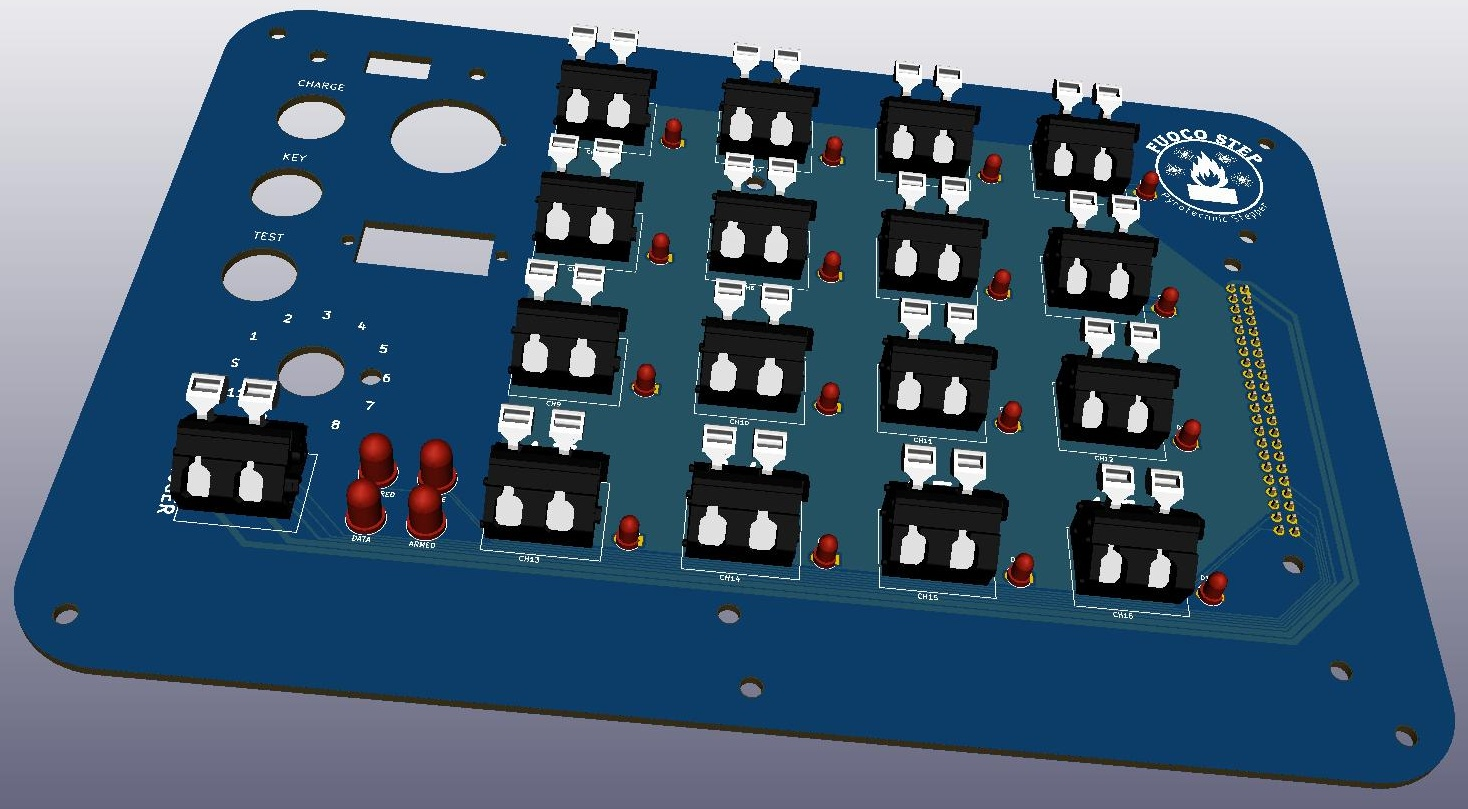
\includegraphics[width=.8\textwidth]{Bilder/panel3d}
					\captionof{figure}{3D-Illustration des gelöteten Panels}
					\label{fig:panel3d}
				\end{center}

				Anschließend müssen die restlichen Löcher in der Platine gefüllt werden:

				\begin{description}
					\item
					      [Drehschalter] Die Schritte zur Konfektionierung des Drehschalters sind in Abbildung~\ref{fig:drehschalter} illustriert. Den Schalter hierzu kopfüber positionieren, um bequem an der Unterseite arbeiten zu können.

					      \begin{figure}
						      \centering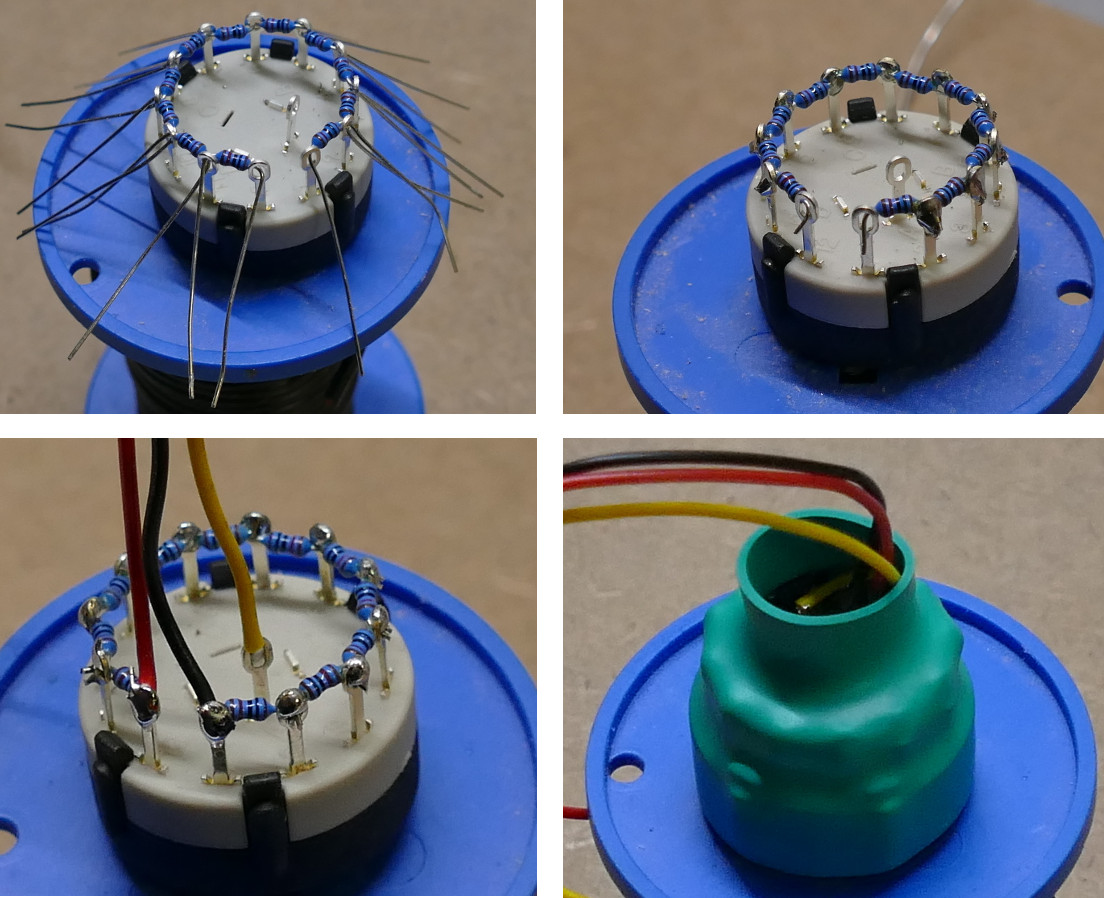
\includegraphics[width=.8\textwidth]{Bilder/Drehschalter}
						      \caption{Konfektionierung des Drehschalters: Stecken der Widerstände, Verlöten der Widerstände, Verlöten der Kabel, Isolierung mittels Schrumpfschlauch (von links oben nach rechts unten)}
						      \label{fig:drehschalter}
					      \end{figure}

					      Zunächst müssen die elf kleinen Widerstände von innen nach außen zwischen den Kontakten 1 und 2, 2 und 3, 3 und 4, \dots, 11 und 12 gesteckt werden, nur die Lücke zwischen 1 und 12 bleibt frei (Bild links oben). Anschließend werden die Drahtpaare an den Pins 2 bis 11 gelötet; 1 und 12 noch nicht verlöten, erst Kabel anbringen (Bild rechts oben). Am Pin 1 ist das kurze schwarze, am Pin 12 das kurze rote und zusätzlich am inneren Pin das kurze gelbe Kabel anzulöten (Bild links unten). Falls ein Multimeter zur Verfügung steht, sollte jetzt kontrolliert werden, ob zwischen rotem und schwarzem Kabelende ein Widerstand im Bereich von \SI{110}{\kilo\ohm} gemessen wird. Falls nicht, alle Lötstellen noch einmal genau überprüfen bzw. nacharbeiten und neu messen. Liegt der Widerstand schließlich im angestrebten Bereich, kann man abschließend den grünen Schrumpfschlauch auf den Schalter ziehen und per Fön erhitzen, wobei die Kabel noch herausstehen sollen (Bild rechts unten).

					      Nun den Schalter in die Platine stecken, festschrauben und die Schalterkappe befestigen. Am Ende müssen dann die drei Kabel auf der Platine festgelötet werden. Hierzu zunächst die Pads kräftig mit Lötzinn vorverzinnen, die Kabel am Ende der Isolierung abknicken, Pad erhitzen und Kabelende in den Zinn drücken: rot bei Pad \enquote{3,3V}, gelb bei Pad \enquote{ADC} und schwarz bei Pad \enquote{GND}. Das Erkalten des Zinns kann ein paar Sekunden dauern, daher das Kabel nicht zu früh loslassen.
					\item
					      [Testschalter] In die Platine stecken und festschrauben
					\item
					      [Schlüsselschalter] In die Platine stecken und festschrauben, dabei darauf achten, dass der rote Punkt am Schalter bei \enquote{Inactive}, der grüne bei \enquote{Armed} liegt.
					\item
					      [Ladebuchse] In die Platine stecken und festschrauben. Vor dem späteren Löten (siehe weiter unten) die Gummiabdeckung öffnen, damit der Gummi durch die Hitze keinen Schaden nimmt!
					\item
					      [Spannungsanzeige] In die Platine stecken und mit den M2-Schrauben und zugehörigen Muttern festschrauben. Orientierung beachten, so dass die Dezimalpunkte, wie in Abbildung~\ref{fig:paneldescription} gezeigt, nach unten weisen.
					\item
					      [Hauptschalter] In die Platine stecken, bis er einrastet (erfordert mehr als nur sanften Druck)
					\item
					      [Micro-USB-Anschluss] Mit den zugehörigen Schrauben festschrauben
					\item
					      [Abdeckung der Lötstellen] Mit den beiden M3x6-Schrauben und passenden Muttern befestigen
				\end{description}

				Die Bedien- und Anzeigeelemente, welche in der Platine verschraubt sind, müssen nun noch mit den entsprechenden Kabeln verbunden werden, die später den Kontakt zur Steuerplatine herstellen.

				Hierfür zunächst die Schrumpfschlauchabschnitte vorbereiten:
				\begin{itemize}
					\item
					      Vom Schrumpfschlauch mit \SI{6,4}{\milli\metre} Durchmesser drei Teile mit je \SI{15}{\milli\metre} Länge abschneiden (für die Hauptschalterkontakte), den Rest in zwei gleiche Hälften zerschneiden (für die Befestigung am Akku).
					\item
					      Aus dem Schrumpfschlauch mit \SI{4,8}{\milli\metre} Durchmesser vier gleichlange Teile herstellen (für die Deans-Verbinder)
					\item
					      Aus dem Schrumpfschlauch mit \SI{3,2}{\milli\metre} Durchmesser sechs gleichlange Teile herstellen (für Ladebuchse, Schlüssel- und Testschalter)
				\end{itemize}

				Beim dreipoligen Crimpgehäuse zunächst die drei kurzen Schrumpfschlauchstücke des Durchmessers \SI{6,4}{\milli\metre} über die losen Kabelenden bis zum Gehäuse schieben. Die Zuordnung zwischen Kabeln und Kontakten ist: Rotes Kabel an den äußeren silbernen Kontakt des Hauptschalters, weißes Kabel an den Mittelkontakt und graues Kabel an den goldenen Kontakt. Dann aus dem abisolierten Teil des Kabels ein \enquote{U} formen, das Kabel durch den zugehörigen Kontakt fädeln und vor dem Verlöten mit einer Zange auf beiden Seiten die Litze an den Kontakt drücken, dann verlöten. Kontakte danach mit den vorher aufgeschobenen Schrumpfschläuchen isolieren.

				Beim achtpoligen Crimpgehäuse zunächst das blaue Kabel mit den beiden inneren Kontakten des Displays verbinden, das benachbarte schwarze Kabel mit dem Außenkontakt wie in Abbildung~\ref{fig:displayloetung} im roten Kreis gezeigt. Hierzu das Litzenbündel beim blauen Kabel in zwei gleich starke Äste aufspalten, verdrillen und vor dem Verlöten sauber in die beiden Löcher einführen. Gut darauf achten, dass zwischen dem mittleren und äußeren Pad kein Kurzschluss entsteht. Zur Sicherheit kann vorsichtig mit dem Cuttermesser zwischen den beiden Pads gekratzt werden.

				\begin{figure}
					\centering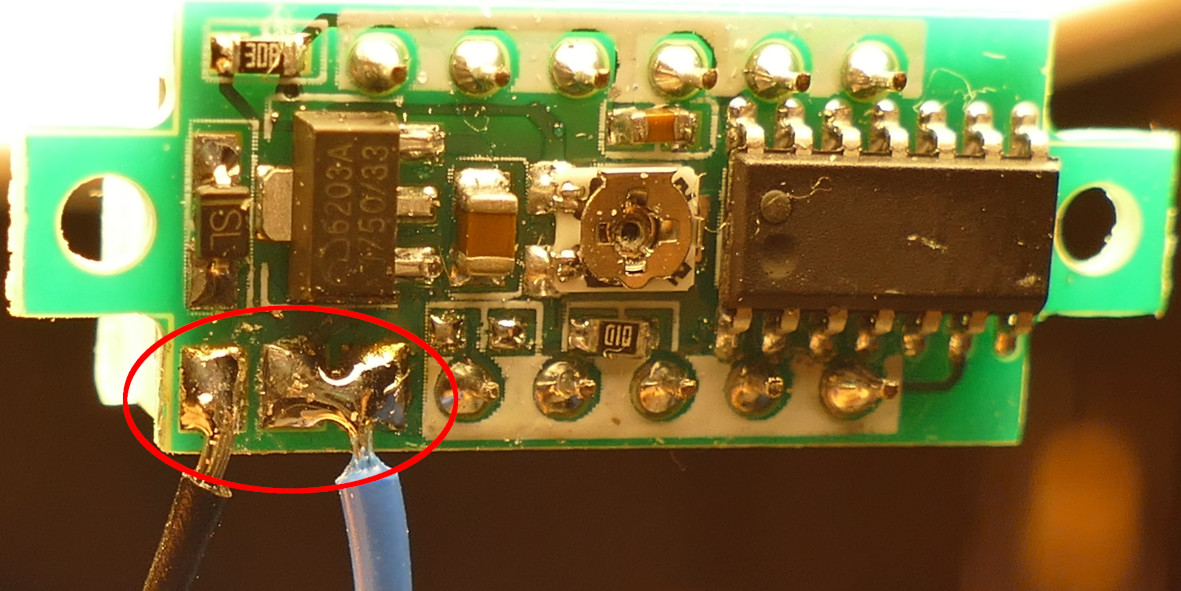
\includegraphics[width=.5\textwidth]{Bilder/displayloetung}
					\caption{Anschluss des Displays zur Spannungsanzeige}
					\label{fig:displayloetung}
				\end{figure}

				Anschließend Schrumpfschläuche des Durchmessers \SI{3,2}{\milli\metre} über die gelben, violetten sowie das rote und übrige schwarze Kabel bis zum Gehäuse schieben, die Durchfädeltechnik wie beim Hauptschalter anwenden und folgendermaßen verlöten: Rotes Kabel an den L-förmigen Kontakt der Ladebuchse, welcher mit dem Stift verbunden ist, schwarzes dickes Kabel an den anderen Kontakt der Ladebuchse. Die beiden violetten Kabel gehören an den Schlüsselschalter, die beiden gelben Kabel an den Testschalter, wobei die Pinzuordnung hier egal ist. Kontakte anschließend mit Schrumpfschlauch isolieren.

				\clearpage
		\section{Basis}
			\subsection*{Bauteilindex}

				Die in der Platine zu verlötenden Teile sind in der folgenden Tabelle aufgeführt:

				\begin{xltabular}
					[l]{\textwidth}{llX}
					Reference & Value/Name             & Package                                                 \\ \hline\hline
					\endhead
					C         &                        &                                                         \\*
					C1        & 100n                   & C\_Disc\_D3.8mm\_W2.6mm\_P2.50mm                        \\
					C2        & 100n                   & C\_Disc\_D3.8mm\_W2.6mm\_P2.50mm                        \\
					C3        & 100n                   & C\_Disc\_D3.8mm\_W2.6mm\_P2.50mm                        \\
					C4        & 100n                   & C\_Disc\_D3.8mm\_W2.6mm\_P2.50mm                        \\
					C5        & 100n                   & C\_Disc\_D3.8mm\_W2.6mm\_P2.50mm                        \\
					C6        & 100n                   & C\_Disc\_D3.8mm\_W2.6mm\_P2.50mm                        \\
					C7        & 100n                   & C\_Disc\_D3.8mm\_W2.6mm\_P2.50mm                        \\
					C8        & 100n                   & C\_Disc\_D3.8mm\_W2.6mm\_P2.50mm                        \\
					C9        & 10u                    & CP\_Radial\_D6.3mm\_P2.50mm                             \\
					C10       & 10u                    & CP\_Radial\_D6.3mm\_P2.50mm                             \\
					C11       & 100n                   & C\_Disc\_D3.8mm\_W2.6mm\_P2.50mm                        \\
					C12       & 100n                   & C\_Disc\_D3.8mm\_W2.6mm\_P2.50mm                        \\
					C13       & 4m7                    & CP\_Radial\_D18.0mm\_P7.50mm                            \\
					C14       & 4m7                    & CP\_Radial\_D18.0mm\_P7.50mm                            \\
					C15       & 100n                   & C\_Disc\_D3.8mm\_W2.6mm\_P2.50mm                        \\
					\hline

					D         &                        &                                                         \\*
					D1        & 1N4001                 & D\_DO-41\_SOD81\_P10.16mm\_Horizontal                   \\
					D2        & 1N4001                 & D\_DO-41\_SOD81\_P10.16mm\_Horizontal                   \\
					\hline

					J         &                        &                                                         \\*
					J1        & Conn\_02x22\_Odd\_Even & PinSocket\_2x22\_P2.54mm\_Vertical                      \\
					J2        & Conn\_01x03            & Molex\_KK-254\_AE-6410-03A\_1x03\_P2.54mm\_Vertical     \\
					J3        & Conn\_01x08            & Molex\_KK-254\_AE-6410-08A\_1x08\_P2.54mm\_Vertical     \\
					\emph{J4} & Conn\_01x05            & PinHeader\_1x05\_P2.54mm\_Vertical                      \\
					\emph{J5} & Conn\_02x05\_Odd\_Even & IDC-Header\_2x05\_P2.54mm\_Vertical                     \\
					\emph{J6} & Conn\_01x02            & PinHeader\_1x02\_P2.54mm\_Vertical                      \\
					\emph{J7} & USB\_B\_Micro          & MIUSB-F5MX-BB-U                                         \\
					\hline

					Q         &                        &                                                         \\*
					Q1        & IRF3708                & TO-220-3\_Vertical                                      \\
					Q2        & IRF3708                & TO-220-3\_Vertical                                      \\
					Q3        & IRF3708                & TO-220-3\_Vertical                                      \\
					Q4        & IRF3708                & TO-220-3\_Vertical                                      \\
					Q5        & IRF3708                & TO-220-3\_Vertical                                      \\
					Q6        & IRF3708                & TO-220-3\_Vertical                                      \\
					Q7        & IRF3708                & TO-220-3\_Vertical                                      \\
					Q8        & IRF3708                & TO-220-3\_Vertical                                      \\
					Q9        & IRF3708                & TO-220-3\_Vertical                                      \\
					Q10       & IRF3708                & TO-220-3\_Vertical                                      \\
					Q11       & IRF3708                & TO-220-3\_Vertical                                      \\
					Q12       & IRF3708                & TO-220-3\_Vertical                                      \\
					Q13       & IRF3708                & TO-220-3\_Vertical                                      \\
					Q14       & IRF3708                & TO-220-3\_Vertical                                      \\
					Q15       & IRF3708                & TO-220-3\_Vertical                                      \\
					Q16       & IRF3708                & TO-220-3\_Vertical                                      \\
					Q17       & BC337                  & TO-92\_Inline\_Wide                                     \\
					Q18       & IRF4905                & TO-220-3\_Vertical                                      \\
					Q19       & BC337                  & TO-92\_Inline\_Wide                                     \\
					Q20       & BC327                  & TO-92\_Inline\_Wide                                     \\
					\hline

					R         &                        &                                                         \\*
					R1        & 10k                    & R\_Axial\_DIN0207\_L6.3mm\_D2.5mm\_P10.16mm\_Horizontal \\
					R2        & 4k7                    & R\_Axial\_DIN0207\_L6.3mm\_D2.5mm\_P10.16mm\_Horizontal \\
					R3        & 150                    & R\_Radial\_Power\_L9.0mm\_W10.0mm\_Px2.90mm\_Py2.40mm   \\
					R4        & 2R2                    & R\_Radial\_Power\_L9.0mm\_W10.0mm\_Px2.90mm\_Py2.40mm   \\
					R5        & 1k5                    & R\_Axial\_DIN0207\_L6.3mm\_D2.5mm\_P10.16mm\_Horizontal \\
					R6        & 270                    & R\_Axial\_DIN0207\_L6.3mm\_D2.5mm\_P10.16mm\_Horizontal \\
					R7        & 1k0                    & R\_Axial\_DIN0207\_L6.3mm\_D2.5mm\_P10.16mm\_Horizontal \\
					R8        & 1k0                    & R\_Axial\_DIN0207\_L6.3mm\_D2.5mm\_P10.16mm\_Horizontal \\
					R9        & 330                    & R\_Axial\_DIN0207\_L6.3mm\_D2.5mm\_P10.16mm\_Horizontal \\
					R10       & 150k                   & R\_Axial\_DIN0207\_L6.3mm\_D2.5mm\_P10.16mm\_Horizontal \\
					R11       & 47k                    & R\_Axial\_DIN0207\_L6.3mm\_D2.5mm\_P10.16mm\_Horizontal \\
					R12       & 1k0                    & R\_Axial\_DIN0207\_L6.3mm\_D2.5mm\_P10.16mm\_Horizontal \\
					R13       & 1k0                    & R\_Axial\_DIN0207\_L6.3mm\_D2.5mm\_P10.16mm\_Horizontal \\
					R14       & 1k0                    & R\_Axial\_DIN0207\_L6.3mm\_D2.5mm\_P10.16mm\_Horizontal \\
					R15       & 1k0                    & R\_Axial\_DIN0207\_L6.3mm\_D2.5mm\_P10.16mm\_Horizontal \\
					R16       & 47                     & R\_Radial\_Power\_L9.0mm\_W10.0mm\_Px2.90mm\_Py2.40mm   \\
					\hline

					RN        &                        &                                                         \\*
					RN1       & 10k                    & R\_Array\_SIP9                                          \\
					RN2       & 10k                    & R\_Array\_SIP9                                          \\
					RN3       & 4k7                    & R\_Array\_SIP9                                          \\
					RN4       & 4k7                    & R\_Array\_SIP9                                          \\
					\hline

					U         &                        &                                                         \\*
					U1        & ATmega328P-PU          & DIP-28\_W7.62mm                                         \\
					U2        & 74HC595                & DIP-16\_W7.62mm                                         \\
					U3        & 74HC595                & DIP-16\_W7.62mm                                         \\
					U4        & LM1084-3.3             & TO-220-3\_Vertical                                      \\
					U5        & SFH620A-3              & DIP-4\_W7.62mm                                          \\
					U6        & MCP6002-xP             & DIP-8\_W7.62mm                                          \\
					U7        & MCP2221\_IP            & DIP-14\_W7.62mm                                         \\
					U8        & XL6009\_Module         & XL6009\_STEP-UP-MODULE                                  \\
					\hline
				\end{xltabular}
				\captionof{table}{Bauteile der Basis}
				\label{tab:bauteilebasis}

			\subsection*{Vorgehensweise}
				Die Bauteile sollten auch hier von klein nach groß eingelötet werden und jeweils bündig auf der Platine aufliegen, sofern nichts anderes vermerkt ist. Eine fertig bestückte Variante ist in Abbildung~\ref{fig:base-eingebaut} auf Seite~\pageref{fig:base-eingebaut} zu sehen:
				\begin{enumerate}
					\item
					      Die kleinen Widerstände \texttt{R1}, \texttt{R2}, \texttt{R5}, \texttt{R6}, \texttt{R7}, \texttt{R8}, \texttt{R9}, \texttt{R10}, \texttt{R11}, \texttt{R12}, \texttt{R13}, \texttt{R14}, \texttt{R15} in der Bauform 0207. Hier spielt die Polarität keine Rolle, allerdings ist auf die Werte zu achten, die anhand der Farbringe festgestellt werden können\footnote{Falls sich jemand genauer für die Kennzeichnung der Widerstände interessiert: jede Farbe symbolisiert eine Zahl, nämlich schwarz=0, braun=1, rot=2, orange=3, gelb=4, grün=5, blau=6, violett=7, grau=8, weiß=9. Der Widerstandswert in Ohm ist bei fünf Ringen folgendermaßen zu lesen: (100*Ring1 + 10*Ring2 + Ring3) * 10$^{\text{Ring4}}$ mit einer Toleranz von Ring5, wobei bei Ring 5 braun=\SI{1}{\percent}, rot=\SI{2}{\percent}, grün=\SI{0,5}{\percent}, blau=\SI{0,25}{\percent}, violett=\SI{0,1}{\percent}, gold=\SI{5}{\percent} und silber=\SI{10}{\percent} bedeutet. Gold und silber können auch als Farben des Rings 4 auftreten, gold=-1, silber=-2. Der kleinste darstellbare Widerstandswert größer \SI{0}{\ohm} mit 1-\%-Toleranz wäre also die Kombination schwarz-schwarz-braun-silber-braun, dies entspricht \SI{0,01}{\ohm}, der größte so darstellbare Wert wäre weiß-weiß-weiß-weiß-braun, also \SI{999}{\giga\ohm}.}. Tabelle~\ref{tab:widerstandswerte} zeigt die Widerstandswerte und ihre farbliche Kennzeichnung.

					      Der \enquote{erste} Ring ist derjenige, der am weitesten außen am Gehäuse angebracht ist, ansonsten den Widerstand so drehen, dass die Farbreihenfolge einer in der Tabelle genannten entspricht, rechts muss immer ein brauner Ring sein.

					      Besondere Vorsicht ist bei den Werten geboten, die sich nur um Zehnerpotenzen, also nur im vierten Ring unterschieden: (\SI{1}{\kilo\ohm} und \SI{10}{\kilo\ohm}, \SI{1,5}{\kilo\ohm} und \SI{150}{\kilo\ohm} sowie \SI{4,7}{\kilo\ohm} und \SI{47}{\kilo\ohm}). Hier darauf achten, dass bei den jeweils kleineren Werten der vierte und fünfte Ring dieselbe Farbe besitzen.

					      \begin{table}
						      \begin{center}
							      \begin{minipage}[b]{.6\textwidth}
								      \begin{tabular}
									      {|r@{\,}l|ccccc|}\hline
									      \multicolumn{2}{|c|}{Wert} & 1. Ring              & 2. Ring               & 3. Ring & 4. Ring              & 5. Ring            \\ \hline\hline
									      270 & \si{\ohm}            & \color{red}rot       & \color{violet}violett & schwarz & schwarz              & \color{brown}braun \\ \hline
									      330 & \si{\ohm}            & \color{orange}orange & \color{orange}orange  & schwarz & schwarz              & \color{brown}braun \\ \hline
									      1   & \si{\kilo\ohm}       & \color{brown}braun   & schwarz               & schwarz & \color{brown}braun   & \color{brown}braun \\ \hline
									      1,5 & \si{\kilo\ohm}       & \color{brown}braun   & \color{green}grün     & schwarz & \color{brown}braun   & \color{brown}braun \\ \hline
									      4,7 & \si{\kilo\ohm}       & \color{yellow}gelb   & \color{violet}violett & schwarz & \color{brown}braun   & \color{brown}braun \\ \hline
									      10  & \si{\kilo\ohm}       & \color{brown}braun   & schwarz               & schwarz & \color{red}rot       & \color{brown}braun \\ \hline
									      47  & \si{\kilo\ohm}       & \color{yellow}gelb   & \color{violet}violett & schwarz & \color{red}rot       & \color{brown}braun \\ \hline
									      150 & \si{\kilo\ohm}       & \color{brown}braun   & \color{green}grün     & schwarz & \color{orange}orange & \color{brown}braun \\ \hline
								      \end{tabular}
								      \vspace{0pt}
							      \end{minipage}
							      %
							      \begin{minipage}[b]{.2\textwidth}
								      \vspace{0pt}
								      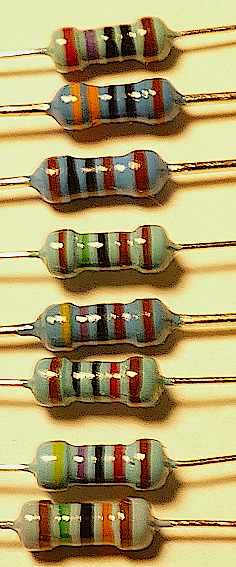
\includegraphics[height=40mm]{Bilder/Widerstaende}
							      \end{minipage}
						      \end{center}
						      \caption{Identifizierung der Widerstandswerte}
						      \label{tab:widerstandswerte}
					      \end{table}
					      Drähte nach dem Einlöten kürzen.

					\item
					      Die beiden Dioden \texttt{D1} und \texttt{D2}, wobei die Orientierung wichtig ist. Drähte nach dem Einlöten kürzen.
					\item
					      Die kleinen 100-nF-Kondensatoren \texttt{C1}, \texttt{C2}, \texttt{C3}, \texttt{C4}, \texttt{C5}, \texttt{C6}, \texttt{C7}, \texttt{C8}, \texttt{C11}, \texttt{C12}, \texttt{C15}, Orientierung spielt keine Rolle. Drähte nach dem Einlöten kürzen.
					\item
					      Den ATmega328P-PU~(\texttt{U1}), die beiden 74HC595~(\texttt{U2}, \texttt{U3}), den SFH620A-3~(\texttt{U5}), den MCP6002~(\texttt{U6}) und den MCP2221-I-P~(\texttt{U7}), dabei unbedingt auf korrekte Orientierung achten. Die größeren Gehäuse besitzen an einer der kurzen Seiten eine halbkreisförmige Vertiefung, die im Bestückungsdruck auf der Platine nachempfunden ist, beim Optokoppler SFH620A-3~(\texttt{U5}) ist Pin~1 durch einen Punkt auf dem Gehäuse markiert und gehört ins quadratische der vier Pads.
					\item
					      Die Buchsenleiste, die im Gegensatz zu den anderen Bauteilen von der Unterseite zu stecken und von der Oberseite zu löten ist
					\item
					      Die Widerstandsnetzwerke \texttt{RN1}, \texttt{RN2}, \texttt{RN3}, \texttt{RN4}. Wichtig: Der Punkt auf dem schwarzen Gehäuse muss jeweils am quadratischen Lötpad liegen. Aufschrift beachten, die beiden Netzwerke mit der Aufschrift \enquote{$\bullet$A472G} gehören an den Rand der Platine neben der Buchsenleiste, die Netzwerke mit der Aufschrift \enquote{$\bullet$A103G} neben die Schieberegister.
					\item
					      Die drei Transistoren \texttt{Q17}, \texttt{Q19} und \texttt{Q20} im Package TO-92. Auf korrekte Zuordnung achten, da \texttt{Q20} trotz gleichem Gehäuse ein anderes Modell, nämlich ein BC3\textbf{2}7 ist als die beiden anderen, bei denen es sich um BC3\textbf{3}7 handelt. Ebenso korrekte Orientierung sicherstellen und nicht mit Gewalt in die Platine drücken. Es sollen ruhig noch ein paar Millimeter Draht auf der Oberseite herausschauen, das schwarze Gehäuse soll nicht aufliegen. Drähte nach dem Einlöten kürzen.
					\item
					      Die Molexkonnektoren \texttt{J2} und \texttt{J3}, die Plastikwand muss jeweils zur Platinenmitte weisen
					\item
					      Das Boost-Modul \texttt{U8}: Zunächst die Stiftleiste in vier einzelne Pins zerlegen, indem mit dem Cuttermesser an den verjüngten Stellen der Stiftleiste Druck ausgeübt wird, und diese von der Oberseite in die vier vorgesehenen Löcher in der Platine stecken, so dass der längere Teil des Stifts nach oben zeigt. Beschriftung auf dem Modul mit Beschriftung auf der Platine abgleichen, das Boost-Modul korrekt orientiert in die vier Stifte einfädeln und auf der Oberseite des Moduls verlöten. Anschließend noch die kurzen Enden der Pins auf der Unterseite der Platine anlöten.
					\item
					      Die Elektrolytkondensatoren \texttt{C9} und \texttt{C10}. Äußerst wichtig: Der Draht an der weißen Markierung am Gehäuse (kennzeichnet den Minus-Pol) muss jeweils in das Loch im weißen Bereich. Drähte nach dem Einlöten kürzen.
					\item
					      Die Feldeffekttransistoren \texttt{Q1} bis \texttt{Q16} und \texttt{Q18} (Vorsicht, Q18 ist ein anderes Modell als die 16 anderen Transistoren!), auf korrekte Orientierung und Beschriftung achten. Beinchen nach dem Einlöten kürzen.
					\item
					      Der Spannungsregler \texttt{U4}, auf korrekte Orientierung achten. Beinchen nach dem Einlöten kürzen.
					\item
					      Die großen 4700-\si{\micro\farad}-Kondensatoren \texttt{C13} und \texttt{C14}, der Draht an der weißen \enquote{-}-Markierung am Gehäuse muss jeweils in das Loch im weißen Bereich. Drähte nach dem Einlöten kürzen.
					\item
					      Die großen Zementwiderstände \texttt{R3}, \texttt{R4} und \texttt{R16} -- die Werte der Widerstände sind auf dem Gehäuse aufgedruckt; darauf achten, die richtigen Werte an der richtigen Stelle einzulöten. Orientierung ist durch verfügbaren Platz und Bestückungsdruck vorgegeben, auch wenn die Polarität bei Widerständen keine Rolle spielt. Die Drähte nehmen nahe am Gehäuse Lötzinn nicht so leicht auf, daher geduldig sein und Lötzinn nachführen, bis sich eine schöne kegelförmige Lötstelle bildet. Drähte nach dem Einlöten kürzen.
				\end{enumerate}

				Die Micro-USB-Buchse \texttt{J7} ist bereits vorbestückt, die beiden Stiftleisten \texttt{J4} und \texttt{J6}, müssen nicht bestückt werden. Auch der Wannenstecker {J5} wird im Normalfall nicht benötigt. Keineswegs verbunden werden dürfen die Kontakte von \texttt{JP1}, da man sonst Ein- und Ausgang des Step-Up-Konverters kurzschließt!

				Abbildung~\ref{fig:base3d} zeigt auch die korrekte Orientierung der Bauteile, allerdings sind die Widerstände ohne Farbcode dargestellt.

				\begin{figure}[H]
					\centering\includegraphics[width=.7\textwidth]{Bilder/base3d}
					\caption{3D-Modell der bestückten Basisplatine}
					\label{fig:base3d}
				\end{figure}

		\section{Batterie}

			Schrumpfschlauchstück mit Durchmesser \SI{4,8}{\milli\metre} über das offene Ende des roten Kabels mit Kabelschuh schieben, Kabel an den oberen T-Balken der Deans-Buchse löten, Lötstelle mit Schrumpfschlauch isolieren. Analog geht man mit dem schwarzen Kabel mit Kabelschuh und dem zweiten Kontakt der Deans-Buchse vor und wiederholt die Prozedur mit den Kabeln ohne Kabelschuhe und dem Deans-Stecker, so dass es folgendermaßen aussehen sollte wie in Abbildung~\ref{fig:deans}.

			\begin{figure}
				\centering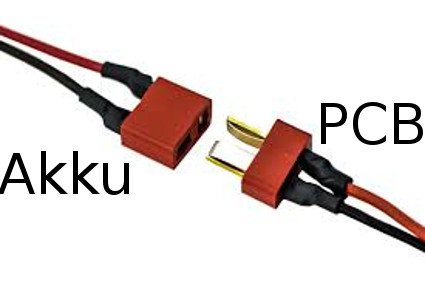
\includegraphics[width=.35\textwidth]{Bilder/deans}
				\caption{Korrekte Verwendung des Deans-Verbinder\-paares}
				\label{fig:deans}
			\end{figure}

			Nun noch das rote mit dem Stecker verbundene Kabel an BATTERY+ und das schwarze an BATTERY- anlöten. Schrumpfschlauch mit Durchmesser \SI{6,4}{\milli\metre} über die Kabelschuhe schieben, Kabelschuhe auf die passenden Batteriekontakte aufschieben (rot an +, schwarz an -), mit etwas Lötzinn fixieren und Kontakte mit Schrumpfschlauch isolieren. Die beiden Deans-Verbinder-Teile jetzt noch nicht zusammenstecken!

		\section{Zusammenbau}
			Nun werden die Einzelteile verbunden, dazu zunächst die Stiftleiste des Panels mit der Buchsenleiste der Basis zusammenstecken.

			Anschließend unter Verwendung der 11-mm-Distanzhülsen die beiden Platinen über die vier Löcher an den Ecken der Basis mit M3x16-Schrauben und zugehörigen Muttern verschrauben. Die Schrauben aus optischen Gründen von der Panelseite stecken, so dass die Muttern später im Gehäuse verschwinden und auf dem Panel die Schraubenköpfe zu sehen sind.

			\begin{figure}
				\begin{center}
					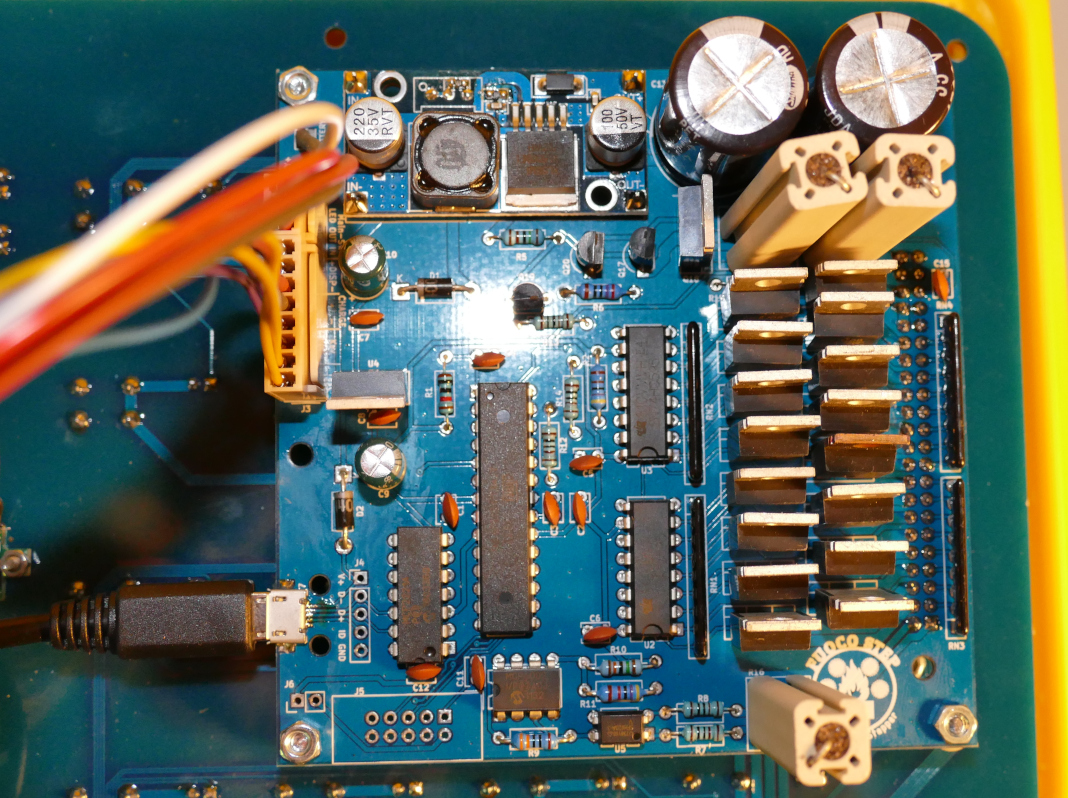
\includegraphics[width=\textwidth]{Bilder/base-eingebaut}
				\end{center}
				\caption{Fertig gelötete und verschraubte Basis}
				\label{fig:base-eingebaut}
			\end{figure}

			Nachdem eine stabile mechanische Verbindung besteht, die beiden Crimpbuchsen und den USB-Stecker an der Basisplatine befestigen. Beim USB-Kabel darauf achten, dass möglichst wenig Zug auf die Platinenbuchse ausgeübt wird; am besten wie in Abbildung~\ref{fig:usbknoten} einen Knoten ins Kabel machen, um es entsprechend kurz zu halten und nicht dauerhaften Zug auszuüben. Die Kabel der Crimpbuchsen und die Batteriekabel können per Kabelbinder zu einem Strang zusammegefasst werden, das erleichtert das spätere Verstauen zwischen Akku und Kofferwand.

			\begin{figure}
				\begin{center}
					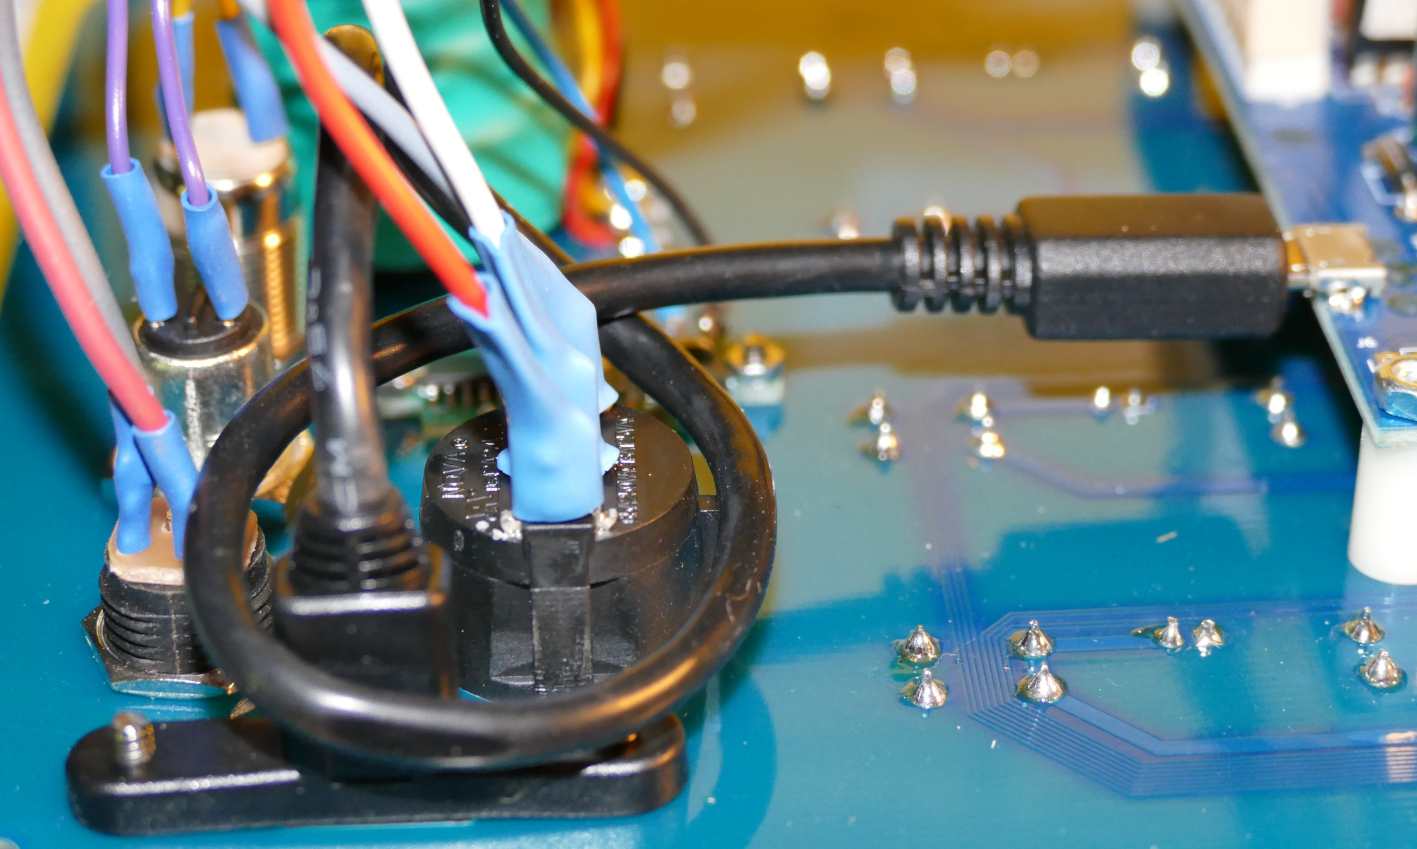
\includegraphics[width=.8\textwidth]{Bilder/usb-knoten}
				\end{center}
				\caption{Verlegen des USB-Anschlusskabels}
				\label{fig:usbknoten}
			\end{figure}

			Die Batterie in den Koffer legen, so dass die Kontakte auf der linken Seite an der vorderen Wand liegen und die verbundenen Platinen passend eingelegt werden können. Die Position des Akkus bezogen auf den Koffer ist in Abbildung~\ref{fig:akkuposition} zu sehen. Zwischen Wand und Akku beträgt der Abstand \SI{37}{\milli\metre}.

			\begin{figure}
				\centering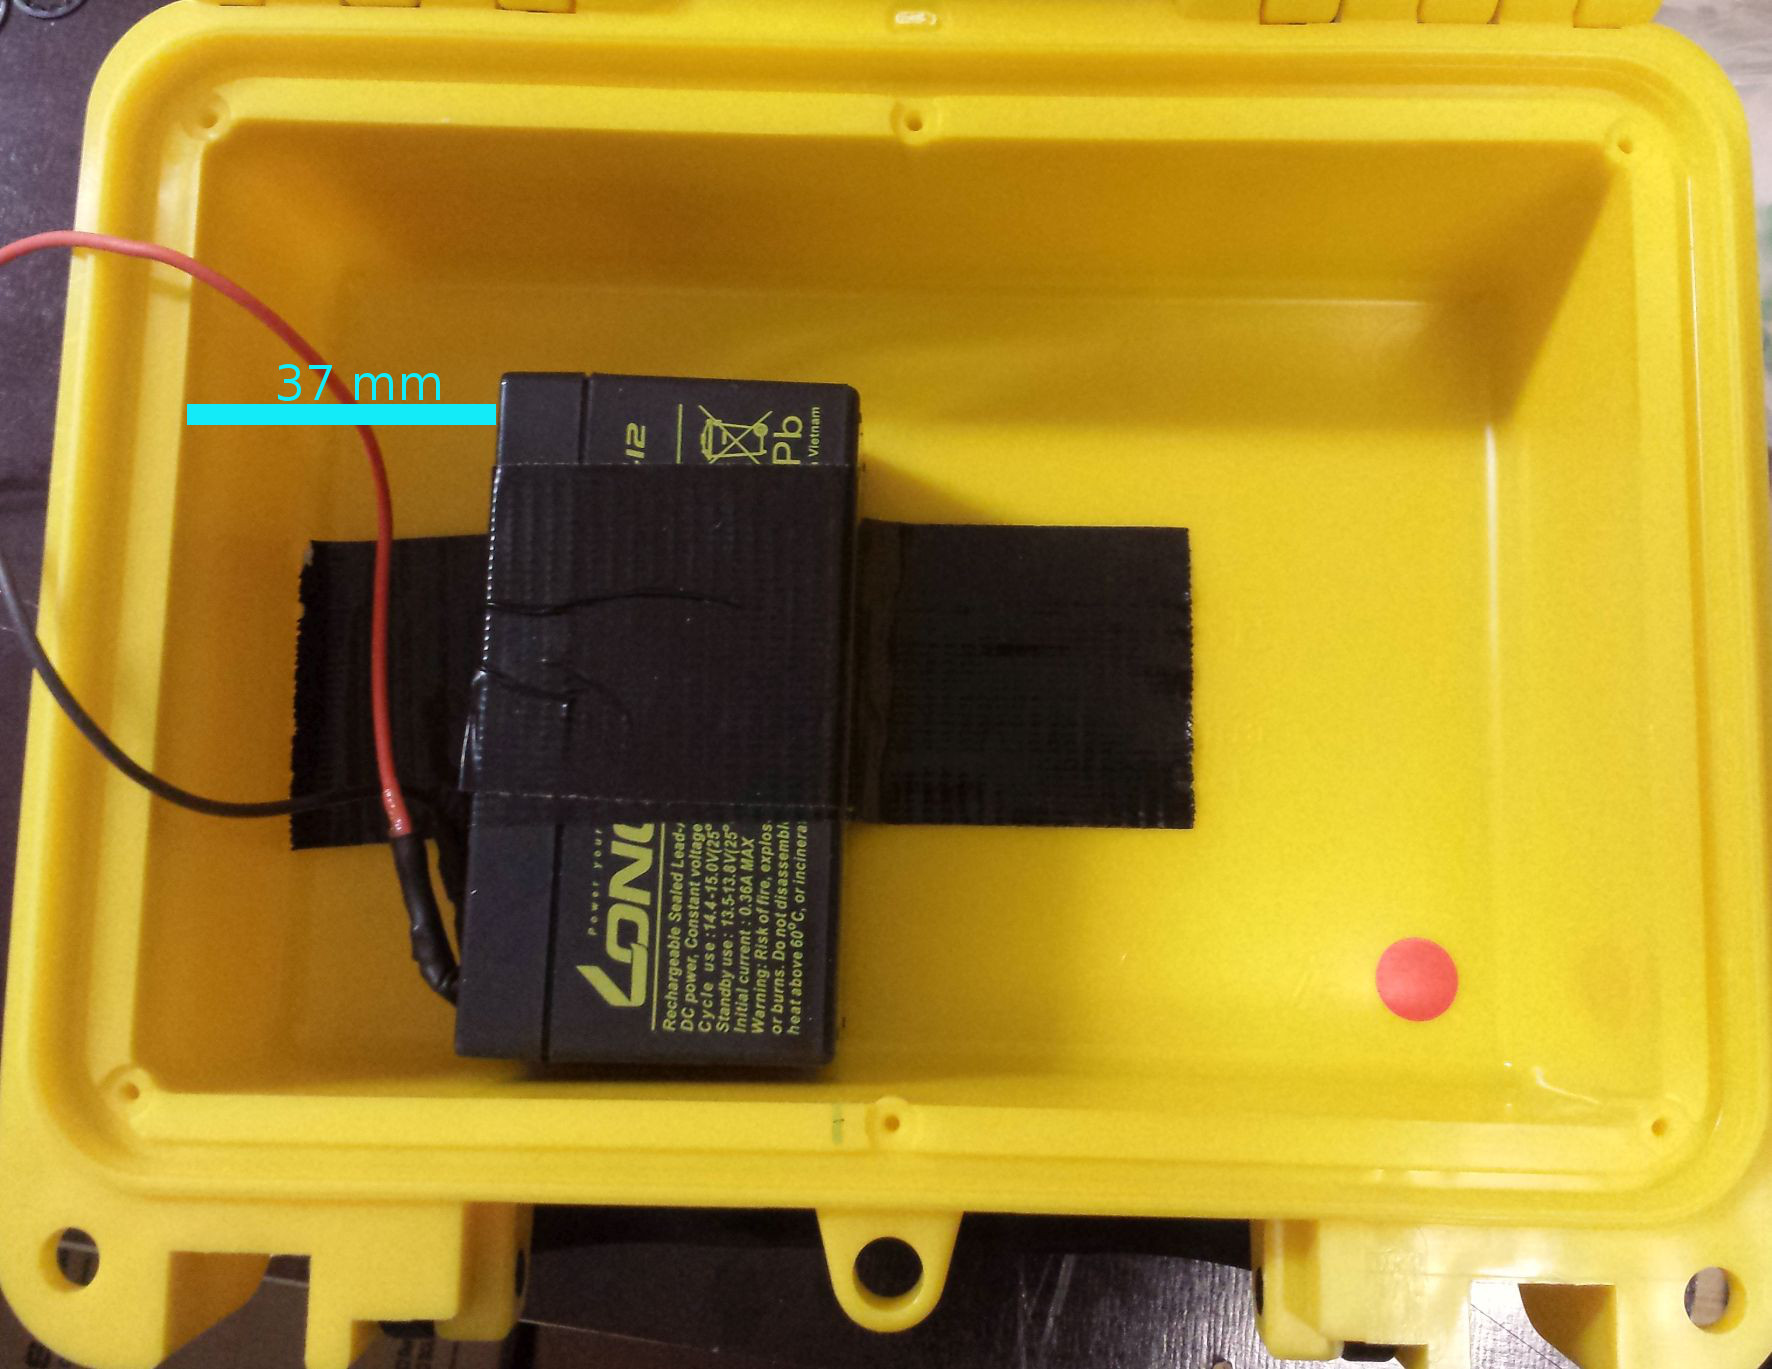
\includegraphics[width=.8\textwidth]{Bilder/Akkuposition}
				\caption{Orientierung und Position des Akkus im Koffer}
				\label{fig:akkuposition}
			\end{figure}

			Es ist nicht allzu viel Platz zwischen der Steckerleiste auf der rechten und dem Unterbau des Drehschalters auf der linken Seite, welche den \enquote{Kanal} für den Akku begrenzen. Ist die korrekte Position für den Akku gefunden, wird er mit einem langen Streifen Gewebeband in seiner Position fixiert (siehe Abbildung~\ref{fig:akkuposition}), wer auf Nummer sicher gehen will, sollte den Akku auf der Unterseite noch mit Teppichklebeband sichern, damit er sich wirklich nicht mehr bewegt.

			Nun die beiden Teile des Deans-Steckverbinders zusammenstecken, die Kabel der Crimpbuchsen zwischen Akku und oberer Wand hindurch führen und das Panel vorsichtig absenken, bis es komplett auf dem Rand zum Liegen kommt und keine Kabel zwischen Panel und Rand eingeklemmt sind. Nun das Panel mit den sechs 3x10-Spaxschrauben am Koffer befestigen.

			\begin{center}
				Der Stepper ist nun einsatzbereit!
			\end{center}

			\cleardoublepage
\part{Bedienungsanleitung}

	\chapter{Funktionsübersicht}

		FUOCO STEP ist ein programmierbarer Stepper/Sequencer/Portexpander mit 16 Kanälen, der während der Show von einem anderen Device über seinen Trigger-Eingang gesteuert wird.

		\begin{figure}[!b]
			\centering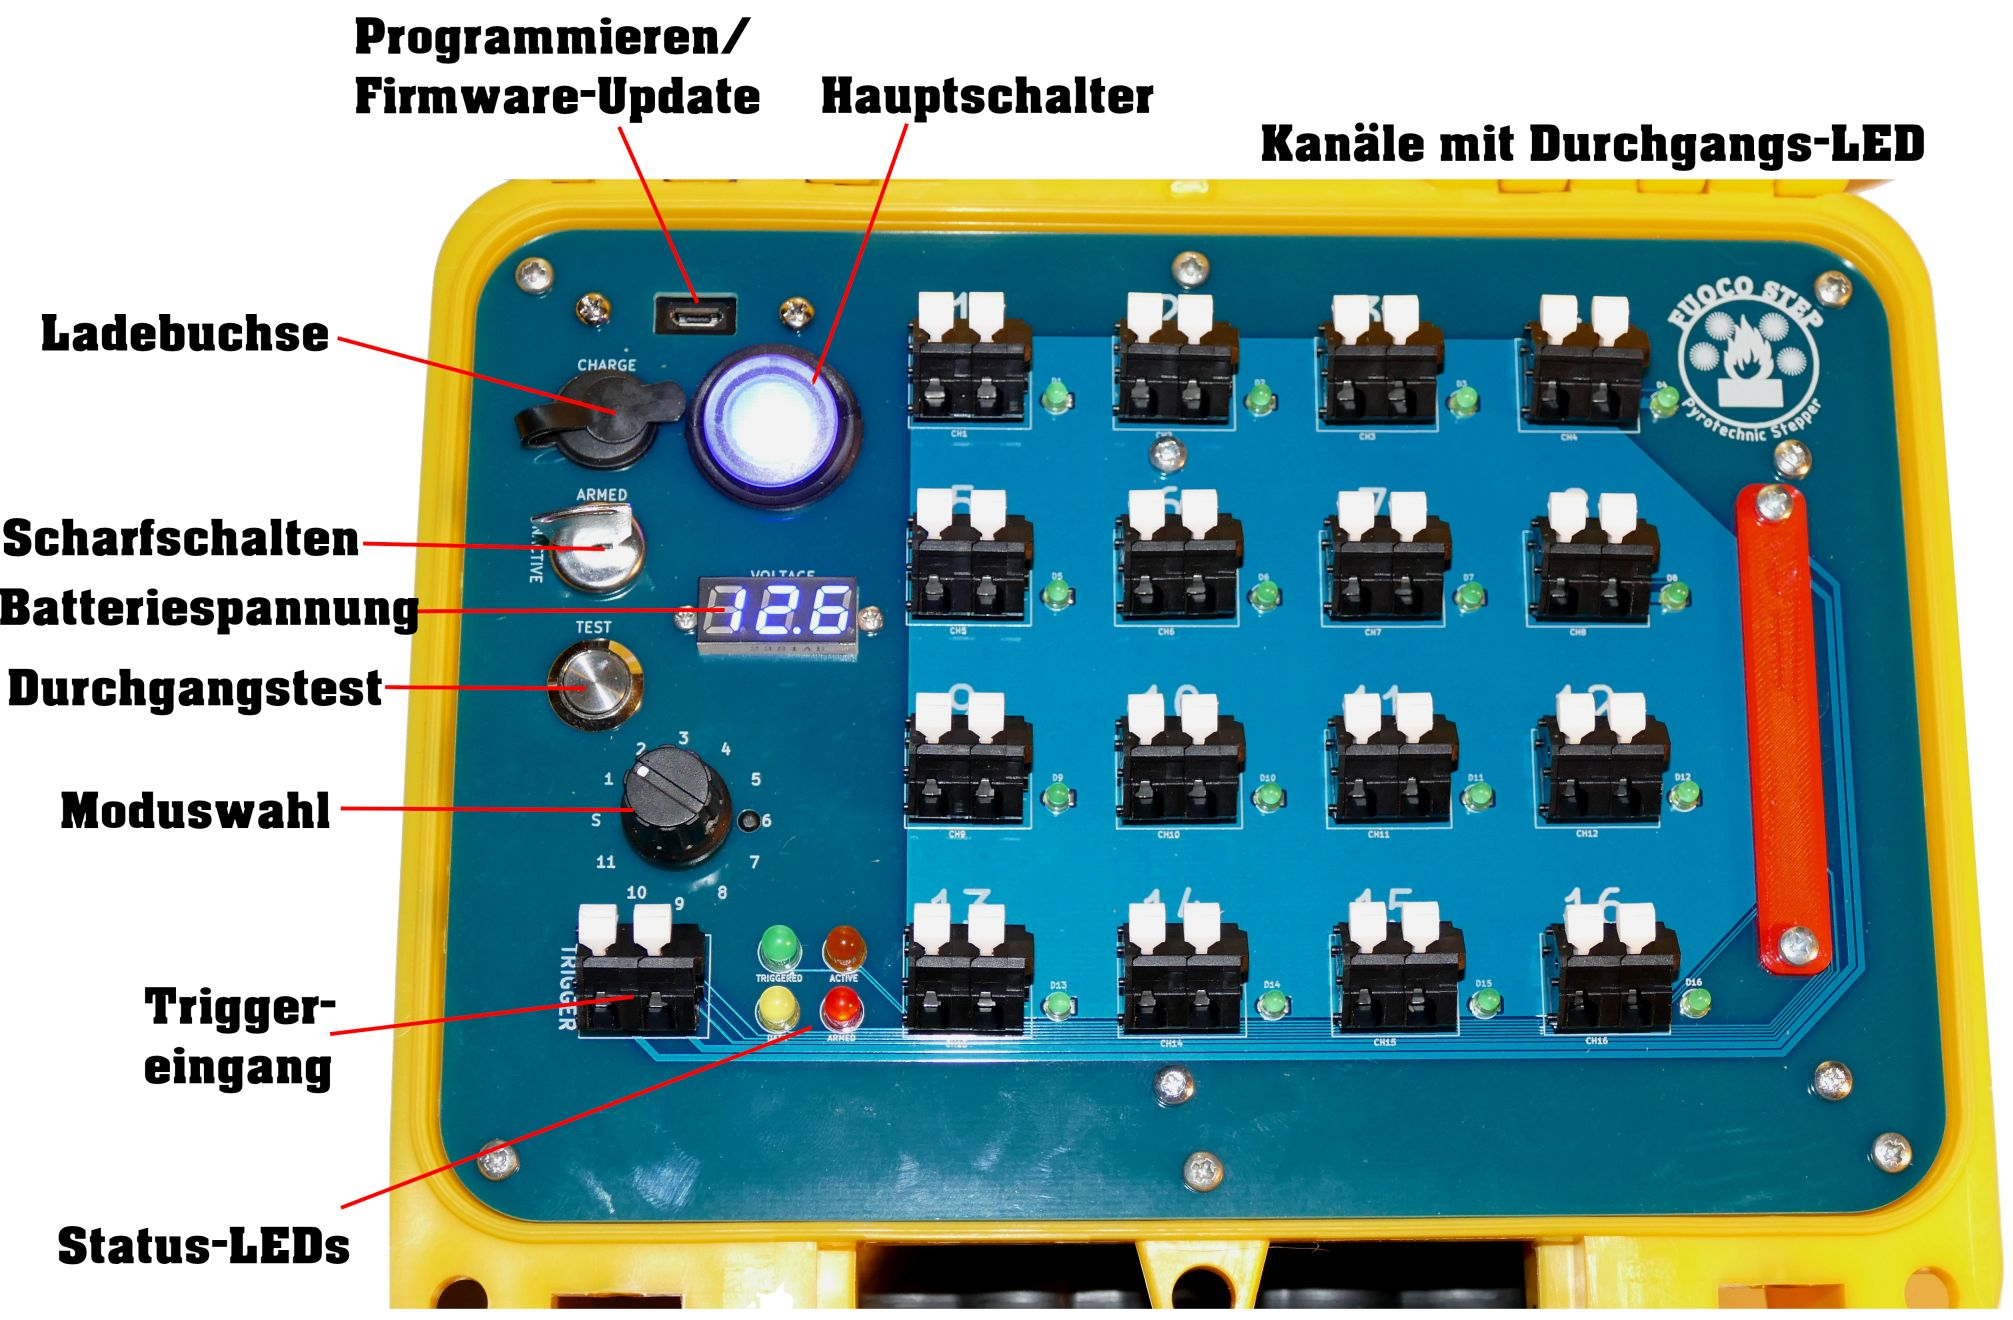
\includegraphics[width=\textwidth]{Bilder/oberflaeche}
			\caption{Übersicht über Bedienoberfläche}
			\label{fig:paneldescription}
		\end{figure}

		Im einfachsten Modus fungiert das Device einfach als Portexpander, stellt also dem triggerenden Zündsystem zusätzliche Kanäle zur Verfügung, indem bei jedem Trigger ein Kanal ausgelöst wird. Beim ersten Aufruf des mit dem Trigger verbundenen Zündkanals wird dann Kanal 1 am Stepper gezündet, beim zweiten Kanal 2, usw.

		Zusätzlich können elf verschiedene Pattern im System hinterlegt werden, bei denen nach dem Trigger die Kanäle zeitgesteuert gezündet werden. Die möglichen Intervalle kann man auf Hundertstel genau zwischen 0,00 Sekunden (gleichzeitige Zündung mehrerer Kanäle) und 9:59,99 Minuten festlegen. Es ist möglich, ein festes Intervall zwischen allen Kanälen zu nutzen, man kann aber auch jedes Intervall einzeln konfigurieren und hat sogar die Möglichkeit, die Sequenz bis zu einem erneuten Trigger zu unterbrechen.

		Die Wahl des aktuellen Patterns erfolgt über einen Drehschalter am Device, die Programmierung sowie eventuelle Firmwareupdates werden via PC, den man via Micro-USB-Kabel an den Stepper anschließt, erledigt. Hierzu kann ein simples Terminal-Programm wie PuTTy genutzt werden, ein graphisches User-Interface, welches in Kapitel~\ref{sec:gui} genauer beschrieben wird, dazu existiert ebenfalls.

		Der Formfaktor des Geräts wurde für einen Seahorse-SE120-Koffer ausgelegt, Spannungsversorgung erfolgt über einen Blei-Gel-Akku (\SI{12}{\volt}/\SI{1,2}{\ampere\hour}), die Zündspannung beträgt 22,5 V~$(\pm\SI{2}{\percent})$, so dass auch längere Reihenschaltungen kein Problem darstellen. Der Triggereingang ist galvanisch vom Rest der Platine getrennt, eine gegenseitige Beeinflussung von Zündanlage und Stepper ist daher ausgeschlossen.

		Weiterhin existieren eine Spannungsanzeige zur Darstellung des aktuellen Batterieladestandes, ein Testschalter, um die Durchgangsprüfung der 16 Kanäle über die kleinen grünen LEDs darzustellen sowie ein Schlüsselschalter zum separaten Scharfschalten des Steppers. Der Akku kann über die integrierte Ladebuchse ohne Aufschrauben mit einem passenden Ladegerät für Blei-Gel-Akkus geladen werden.

		Die Bedienoberfläche unterteilt sich wie in Abbildung~\ref{fig:paneldescription} gezeigt. Auf die einzelnen Funktionen wird in den folgenden Abschnitten eingegangen.

		\section{Hauptschalter}

			Hiermit wird FUOCO STEP ein- und ausgeschaltet. Im eingeschalteten Zustand leuchtet die in den Schalter integrierte LED. Zu beachten ist, dass auch bei ausgeschaltetem Hauptschalter bei gleichzeitig verbundenem USB-Kabel der Logikteil des Steppers mit Strom versorgt, die Zündspannung aber nicht generiert wird. Für die Programmierung muss also der Hauptschalter nicht zwingend eingeschaltet sein.

		\section{Batterieanzeige}

			Bei eingeschaltetem Hauptschalter aktiviert sich die Spannungsanzeige und zeigt nach kurzer Wartezeit die gemessene Batteriespannung des Blei-Gel-Akkus an. Für einen stabilen Betrieb sollte der Wert stets im Bereich von \SI{12}{\volt} oder höher liegen, ansonsten sollte die Batterie nachgeladen werden.

		\section{Ladebuchse}

			Der innere Stift ist unmittelbar mit dem Pluspol des Akkus, der äußere Ring mit dem Minuspol des Akkus verbunden. Um das Ladegerät, z.B. ein H-TRONIC AL800, ungestört arbeiten zu lassen, sollte nur im ausgeschalteten Zustand geladen werden.

		\section{Durchgangstest}

			Ist dieser Schalter gedrückt, versucht die Anlage, einen geringen Strom, der sicher nicht zur Auslösung der Anzünder führt, auf allen Kanälen fließen zu lassen. Das Leuchten der zugehörigen grünen 3-mm-LED signalisiert, dass auf dem entsprechenden Kanal ein Strom fließen kann. Auf diese Weise können Kabelbrüche oder nicht-leitende Verbindungen detektiert werden, eine echte Widerstandsmessung des Kanals findet jedoch nicht statt. Der Testschalter hat keinen Einfluss auf den Zündvorgang, es kann also mit gedrücktem oder ungedrücktem Testschalter gezündet werden.

		\section{Scharfschalten}

			Als zusätzliche Sicherheitsmaßnahme muss der Stepper mit dem Schlüsselschalter separat scharfgeschaltet werden. Wenn das System scharf ist, wird dies durch die dauerhaft leuchtende rote Status-LED (Armed) signalisiert.

		\section{Modusauswahl}
			Der Drehschalter besitzt zwölf Positionen, den Single-Trigger-Modus \enquote{S} sowie die programmierbaren Positionen 1-11. Die Schalterposition wird erfasst, wenn der Schlüsselschalter auf scharf geschaltet wird, eine nachträgliche Drehung hat zunächst keine Wirkung. Über die Bedienoberfläche können jeweils für die aktuell eingestellte Drehschalterposition der Intervallmodus (fest/variabel) sowie die Intervallzeiten festgelegt werden. Näheres dazu in Kapitel~\ref{sec:gui}.

		\section{Triggereingang}
			Über diese Klemme wird der Stepper gestartet, sofern er zuvor scharfgeschaltet wurde. Die Polarität am Eingang spielt keine Rolle, das triggernde Gerät muss mindestens \SI{200}{\milli\ampere} über \SI{47}{\ohm} liefern können, um den Stepper auszulösen.

		\section{Kanalklemmen}
			Hier werden die Anzünder für die einzelnen Kanäle angeschlossen. Die Reihenfolge der Kanäle kann nicht beeinflusst werden, es wird also immer zuerst Kanal 1, dann Kanal 2, usw. ausgelöst. Aufgrund der Zündspannung von \SI{22,5}{\volt} sind längere Reihenschaltungen bis zu zehn Anzündern in Reihe pro Kanal möglich. Die rechts neben den Klemmen befindlichen LEDs signalisieren Durchgang auf dem jeweiligen Kanal, sofern der Testschalter gedrückt ist.

		\section{Status-LEDs}
			Diese vier LEDs signalisieren wesentliche Zustände des Systems.
			\begin{description}
				\item [Gelb/Data] Diese LED leuchtet, während Daten über USB mit dem Rechner ausgetauscht werden
				\item [Rot/Armed] Durch diese LED wird signalisiert, dass der Stepper scharfgeschaltet ist
				\item [Grün/Triggered] Diese LED zeigt an, dass das System getriggert wurde und aktuell eine Sequenz läuft
				\item [Orange/Active] Diese LED leuchtet, solange mindestens ein Kanal aktiv ist
			\end{description}

		\section{Programmieranschluss}
			Durch Anschließen eines Micro-USB-Kabels kann der Stepper über diese Schnittstelle programmiert werden. Dies ist im Detail im Kapitel~\ref{sec:gui} genau beschrieben. Auch Firmware-Updates sind über diesen Anschluss durchführbar.

	\chapter{Programmierung}
		\label{sec:gui}
		\section{Treiberinstallation}
			Idealerweise erkennt Windows beim Anschließen das Gerät von selbst, installiert einen Treiber und stellt es als COM-Port (Serielles USB-Gerät) zur Verfügung.

			Sofern kein Treiber installiert werden kann und das Gerät als \enquote{MCP2221 USB-I2C/UART Combo} unter andere Geräte einsortiert wird und das Ausrufezeichen auf gelbem Grund signalisiert, dass es nicht korrekt funktioniert, muss der entsprechende Treiber einmalig folgendermaßen manuell installiert werden:
			\begin{enumerate}
				\item Die gepackten Treiber von \url{http://ww1.microchip.com/downloads/en/DeviceDoc/MCP2221 Windows Driver 2014-10-09.zip} herunterladen und in einen bekannten Ordner entpacken, den man sich merken sollte
				\item Den Geräte-Manager mit Administratorrechten öffnen
				\item Einen Rechtsklick auf \enquote{MCP2221 USB-I2C/UART Combo} tätigen und \enquote{Treibersoftware aktualisieren} wählen.
				\item Option \enquote{Auf dem Computer nach Treibersoftware suchen} wählen
				\item Auf \enquote{Aus einer Liste von Gerätetreibern auf dem Computer auswählen} klicken
				\item Falls sich nun ein Fenster öffnet, welches sagt \enquote{Wählen Sie den Gerätetyp aus der Liste aus.}, einfach \enquote{Alle Geräte anzeigen} wählen und \enquote{Weiter} klicken
				\item Unten rechts auf die Schaltfläche \enquote{Datenträger\dots} klicken
				\item Im sich nun öffnenden Fenster auf \enquote{Durchsuchen\dots} klicken und zum Ordner, welcher die beiden Treiberdateien enthält, navigieren
				\item Die Datei \enquote{mchpcdc.inf} auswählen und auf \enquote{Öffnen} klicken, im anschließenden Fenster den gewählten Pfad mit \enquote{OK} bestätigen.
				\item Jetzt den Eintrag \enquote{USB-Serial-Port} im Fenster auswählen, auf \enquote{Weiter} klicken und sämtliche Nachfragen bestätigen bzw. Installationen erlauben.
				\item Man sollte die Meldung \enquote{Installation abgeschlossen} erhalten und den Stepper fortan ansprechen können
			\end{enumerate}

		\section{Oberfläche}
			\subsection{Hauptfenster}
				Über die Programmieroberfläche \enquote{stepsetter.exe} ist es möglich, die Steppereinstellungen zu modifizieren. Hierzu muss der passende COM-Port ausgewählt und zunächst die Einstellung des aktuell eingestellten Kanals ausgelesen werden.

				\subsubsection*{Rücksetzen auf Standard}
					Es kann immer nur der Kanal bearbeitet werden, welcher gerade am Stepper per Drehschalter eingestellt ist, Ausnahme ist das Rücksetzen aller Kanäle durch Klick auf \enquote{Standardwerte wiederherstellen}. Bei dieser Aktion werden \underline{alle} Kanäle zurückgesetzt auf festen Intervallmodus mit den Intervallen aus Tabelle~\ref{tab:standardintervalle}.

					\begin{figure}
						\begin{center}
							\begin{xltabular}
								[c]{\textwidth}{c|*{11}c}
								Schalterposition & 1   & 2   & 3   & 4    & 5    & 6    & 7    & 8    & 9    & 10   & 11   \\ \hline
								Intervall (s)    & 2.5 & 5.0 & 7.5 & 10.0 & 12.5 & 15.0 & 17.5 & 20.0 & 25.0 & 30.0 & 40.0
							\end{xltabular}
						\end{center}
						\caption{Standardintervalle des Steppers}
						\label{tab:standardintervalle}
					\end{figure}

					Dies ist auch die einzige Änderung, die bei Schalterstellung \enquote{S} getätigt werden kann, ansonsten werden Eingaben ignoriert, solange der Drehschalter auf \enquote{S} zeigt.

				\subsubsection*{Step-Modus einstellen}

					Schalterstellung \enquote{S} repräsentiert den den Einzelschussmodus, bei dem mit jedem Triggersignal ein Kanal abgefeuert wird. Die maximale Wiederholrate ist dabei von der auslösenden Zündanlage bzw. deren Zündpulslänge abhängig. Bei Cobra dauert ein Puls typischerweise \SI{100}{\milli\second}, ein erneutes Triggern weniger als \SI{100}{\milli\second} nach dem ursprünglichen Trigger würde vom Stepper nicht erkannt und ignoriert werden!

					Für alle anderen Stellungen als \enquote{S} kann der Step-Modus auf eine der beiden Varianten \enquote{Fest} oder \enquote{Variabel} festgelegt werden: Bei \enquote{Fest} ist das Intervall zwischen allen 16 Kanälen identisch, \enquote{Variabel} bietet die Möglichkeit, jedes einzelne Intervall individuell zu konfigurieren. Über die Schaltfläche \enquote{Modus setzen} kann zwischen den beiden Varianten umgeschaltet werden, im Modus \enquote{Fest} bleiben die Intervalle $2-15$ ausgegraut. Nach dem Klick auf \enquote{Modus setzen} im Anschluss an den Schreibvorgang unmittelbar ein Auslesevorgang durchgeführt, so dass die angezeigten Daten die tatsächlichen Einstellungen wiedergeben.

				\subsubsection*{Intervalle festlegen}

					Kanal 1 wird immer unmittelbar beim Triggersignal ausgelöst, Intervall~1 legt also fest, wie viel Zeit zwischen dem Auslösen der Kanäle 1 und 2 vergehen soll, Intervall~2 die Zeit zwischen Kanal 2 und 3, usw. Dementsprechend legt Intervall X die Pause vor Kanal X+1 fest und es ergeben sich bei 16 Kanälen 15 Intervalle.

					Die Eingabe der Zeiten erfolgt typischerweise im Format \enquote{MM:SS.hh} mit Minuten, Sekunden und Hundertsteln, wobei statt des Punktes zwischen Sekunden und -bruchteilen auch das deutsche Dezimalkomma genutzt werden kann. Zahleneingaben ohne Doppelpunkt werden als Sekunden interpretiert, die Eingabe \enquote{1:10.20} beschreibt demnach dasselbe Intervall wie \enquote{70,2}. Bei Eingaben von mehr als zwei Nachkommastellen werden Eingaben abgeschnitten. Möchte man auf ein Triggersignal warten, schreibt man \enquote{T} ins entsprechende Feld. Steht beispielsweise ein \enquote{T} hinter Intervall~5, bedeutet dies, dass vor dem Abfeuern von Kanal~6 wieder auf einen Trigger gewartet wird. Hilfreich kann hier auch das Zusatzfenster \enquote{Absolutzeiten} sein, um das es in Abschnitt~\ref{sec:absolutzeiten} geht.

					Ungültige Eingaben, die andere Zeichen als die Ziffern 0-9, höchstens einen Doppelpunkt, höchstens einen Punkt oder ein Koma oder das Wort \enquote{Trigger} in allen Groß-, Klein- und Abkürzungsformen enthalten, werden ignoriert, Zeitwerte größer als 9:59.99 werden automatisch zu \enquote{Trigger} gewandelt. Da nach jedem Schreibvorgang, den man mit \enquote{Intervall(e) setzen} auslöst, automatisch ein Auslesevorgang durchgeführt wird, kann immer direkt nachvollzogen werden, ob die Eingabe den gewünschten Effekt hatte.

					Abbildung~\ref{fig:beispielsequenz} zeigt ein Beispiel für eine variable Stepsequenz, die immer vier Effekte in kurzer Folge auslöst, ehe für die nächste Abfolge auf einen Trigger gewartet wird. Die letzten beiden Kanäle werden gemeinsam geschossen.

					\begin{figure}[tb]
						\centering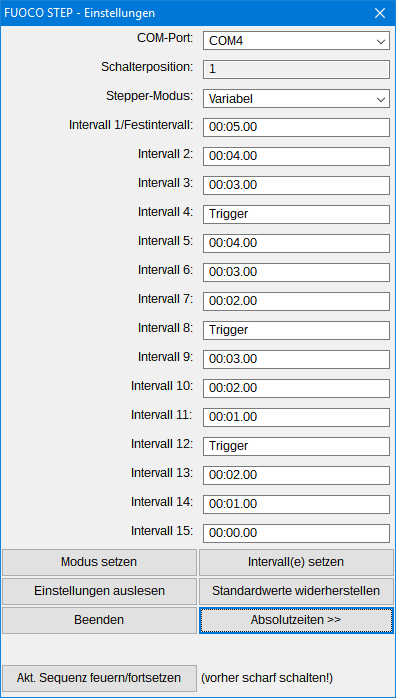
\includegraphics[width=.5\textwidth]{Bilder/beispielshow}
						\caption{Beispielsequenz}
						\label{fig:beispielsequenz}
					\end{figure}

				\subsubsection*{Sequenz feuern oder fortsetzen}

					Mit dieser Taste ist es möglich, die derzeit aktive Einstellung auszulösen, das Verhalten des Steppers ist dabei absolut identisch zu einem tatsächlichen Triggersignal: Ist der Stepper nicht scharf geschaltet, hat ein Druck dieser Taste keinen Effekt, ist er scharf geschaltet, wird die aktuelle Sequenz gestartet oder fortgesetzt und die Kanäle auch tatsächlich ausgelöst. Für einen reinen Testlauf also unbedingt vorher alle Anzünder entfernen!

			\subsection{Zusatzfenster Absolutzeiten}
				\label{sec:absolutzeiten}
				Das Zusatzfenster \enquote{Absolutzeiten} soll ein bequemes Umrechnen von absoluten Zündzeiten, wie man sie in einer Software wie PyroIgnitionControl oder PYROTHEK festlegt, in die von FUOCO~STEP benötigten Intervallzeiten zwischen den einzelnen Kanälen ermöglichen.

				Hierzu können die Werte in der zweiten Spalte eingefügt und die Zeitabstände der einzelnen Kanäle durch Klick auf \enquote{Berechne Intervalle} ermittelt werden. Über \enquote{Werte ins Hauptfenster} können diese Intervallzeiten ins Hauptfenster übertragen werden. Es ist darauf zu achten, dass die aktuelle Schalterposition im passenden Modus konfiguriert sein muss. Ist der feste Intervallmodus eingestellt, wird nur der erste Intervallwert ins Hauptfenster kopiert, beim variablen Intervallmodus alle nicht-leeren Felder. Nach Übertragung ins Hauptfenster müssen die Werte noch durch \enquote{Intervalle setzen} ins Gerät geschrieben werden, um die berechneten Intervalle nutzen zu können.

				Abbildung~\ref{fig:beispielabsolut} zeigt anhand der Intervalle aus der obigen Beispielsequenz die Funktionsweise des Absolut\-zeiten-Fensters. Da die Kanalreihenfolge nicht veränderbar ist, muss jeder Kanal zur selben Zeit oder später beginnen als sein Vorgänger.

				Für die getriggerten Kanäle 1, 5, 9 und 13 wurden hier vor dem Klick auf \enquote{Werte aus Hauptfenster} Zeiten vorgeben, um die absoluten Zündzeiten mit der imaginären Showdatei abgleichen zu können. Ohne Zeitvorgabe würde standardmäßig ein Intervall von einer Minute auf die Absolutzeit des Vorgängers addiert, was für die korrekte Intervallberechnung aber keine Rolle spielt, da Zeitabstände nur bei nicht durch Trigger ausgelösten Kanälen von Bedeutung sind und die Absolutzeiten lediglich der Veranschaulichung für den Anwender dienen.

				\begin{figure}[tb]
					\begin{center}
						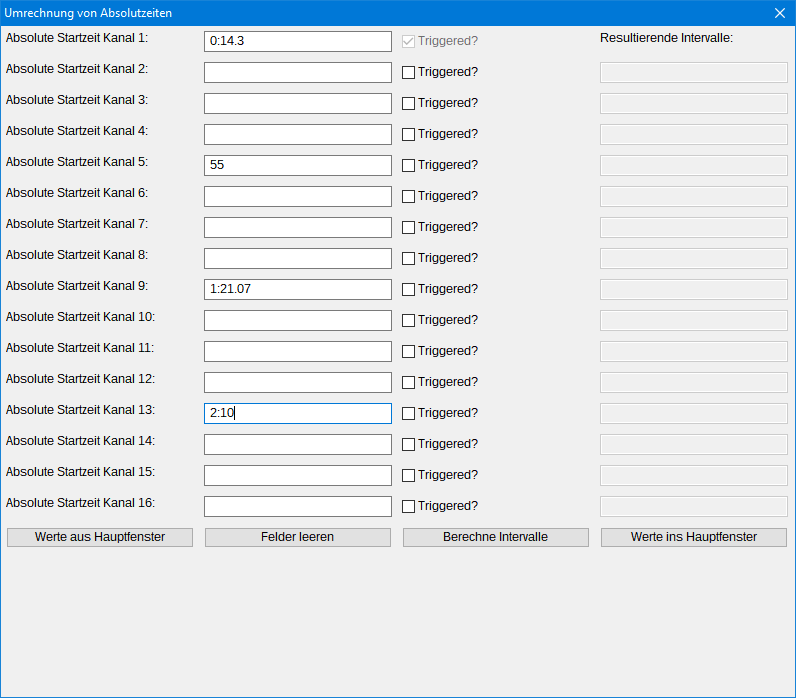
\includegraphics[width=.8\textwidth]{Bilder/beispielzeitvorgabe}{\\}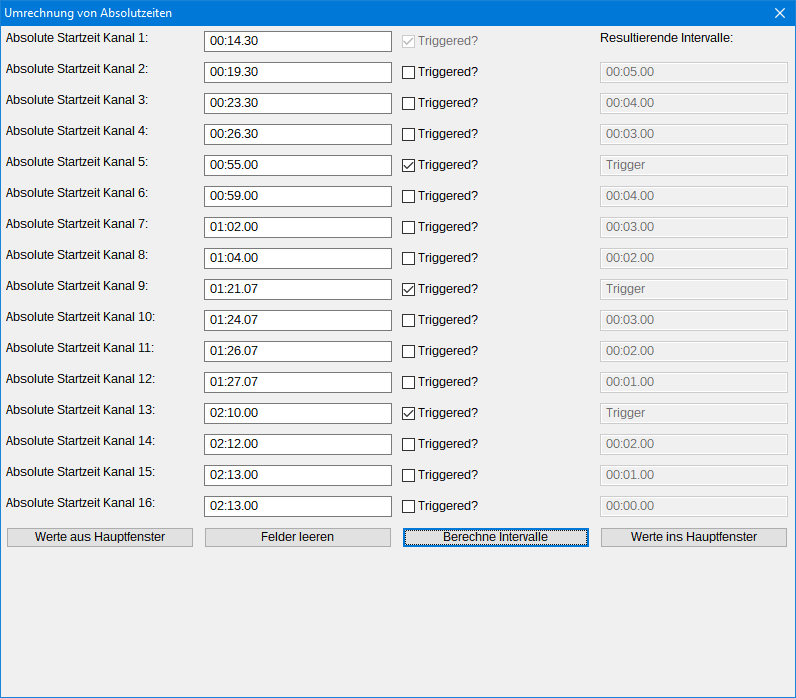
\includegraphics[width=.8\textwidth]{Bilder/beispielabsolut}
					\end{center}
					\caption{Beispiel für die Verwendung des Absolutfensters mit Zeitvorgabe und Intervallberechnung}
					\label{fig:beispielabsolut}
				\end{figure}

				Das Fenster \enquote{Absolutzeiten} kann auch dazu genutzt werden, Einstellungen von einer Schalterstellung auf eine andere zu übertragen. Hierzu die Einstellungen bei der zu kopierenden Schalterposition auslesen und dann nacheinander die Buttons \enquote{Absolutzeiten}, \enquote{Werte aus Hauptfenster} und \enquote{Berechne Intervalle} klicken. Nun die neue Schalterposition auswählen, auslesen, falls nötig den passenden Modus setzen und schließlich durch Klick auf \enquote{Werte ins Hauptfenster} die zu kopierenden Einstellungen setzen.

		\section{Terminal}

			Kann oder will man die graphische Oberfläche nicht nutzen, besteht auch die Möglichkeit, über ein einfaches Terminalprogramm wie \texttt{Putty}\footnote{\url{https://the.earth.li/~sgtatham/putty/latest/w32/putty.exe}} eine serielle Verbindung zu FUOCO STEP aufzubauen und Stepsequenzen zu programmieren. Hierzu ist der Name des COM-Ports zu ermitteln~(COM1, COM2, \dots), unter dem sich FUOCO STEP am Rechner anmeldet, die nötigen Parameter der seriellen Verbindung sind in Tabelle~\ref{tab:seriell} aufgeführt.

			\begin{table}
				\begin{center}
					\begin{xltabular}[c]{7cm}{X|l}
						\hline
						Einstellung      & Wert  \\
						\hline
						Bits pro Sekunde & 9600  \\
						Datenbits        & 8     \\
						Parität          & keine \\
						Stoppbits        & 1     \\
						Flusssteuerung   & keine \\ \hline
					\end{xltabular}
					\caption{Konfiguration der seriellen Schnittstelle}
					\label{tab:seriell}
				\end{center}
			\end{table}

			Diese Einstellungen können händisch in Putty vorgenommen werden, alternativ ist es auch möglich, sie in einer Verknüpfung direkt auf der Kommandozeile zu übergeben, wobei Anwendungspfad und Nummer des COM-Ports (hier 1) entsprechend angepasst werden müssen:
			\begin{center}
				\verb|"c:\programme\putty\putty.exe" -serial com1 -sercfg 9600,8,1|
			\end{center}

			Die Befehle, um FUOCO STEP via Terminal bedienen zu können, lauten:

			\begin{center}
				\begin{xltabular}
					[c]{\textwidth}{p{2.5cm}X}
					\hline
					Befehl  & Bedeutung                                                                                                       \\
					\hline
					list    & Auflisten der aktuellen Einstellungen für alle Stepsequenzen, aktuell aktive Schalterstellung ist gelb markiert \\
					edit    & Verändern der Einstellungen~-- Modus oder Intervall(e)~-- für die aktuelle Schalterstellung                     \\
					trigger & Auslösen eines Software-Triggers, startet, sofern scharfgeschaltet, die aktuell aktive Sequenz                  \\
					igniter & Auswahl des Anzündertyps                                                                                        \\
					cls     & Terminalbildschirm leeren                                                                                       \\
					kill    & Reboot von FUOCO STEP                                                                                           \\
					default & Zurücksetzen der Stepperintervalle auf die Standardeinstellung                                                  \\
					\hline
				\end{xltabular}
				\captionof{table}{Terminalbefehle zur Bedienung von FUOCO STEP}
				\label{tab:commands}
			\end{center}

	\chapter{Softwarepaket}

		\section{Herunterladen der Dateien}

			Alle Dateien zu FUOCO STEP liegen in einem Git-Repository unter \url{https://github.com/fixxl/fuocostep}. Um den aktuellen Stand von Firmware, Bootloader, Bedienoberfläche und Handbuch herunterzuladen, kann folgender Link genutzt werden:
			\begin{center}
				\url{https://github.com/fixxl/fuocostep/archive/master.zip}
			\end{center}
			Im Paket sind zusätzlich der komplette Quellcode sowie das Aktualisierungsprogramm für die Firmware enthalten.

			Wer mit der Nutzung des Versionierungstools Git vertraut ist, kann natürlich das Repository auf seine Festplatte klonen und hat dann den Vorteil, nicht immer das komplette Paket herunterladen zu müssen, sondern gezielt nur die aktualisierten Dateien zu beziehen.

		\section{Firmware-Update}

			Die Firmware ist das \enquote{Betriebssystem} von FUOCO STEP. Wie bei allen Systemen kann es hin und wieder nötig sein, neue Funktionen, welche dem Bedienkomfort und/oder der Sicherheit dienen, einzubauen oder Fehler, welche erst im Betrieb bemerkt werden, auszumerzen. Damit dafür der Koffer nicht hin und her geschickt und aufgeschraubt werden muss, ist eine Aktualisierung der Firmware bequem über USB möglich.

			Im Softwarepaket ist hierfür im Unterverzeichnis \enquote{Firmware-Updater} die Anwendung \enquote{UpdateLoader-win32} enthalten, die Ausführung eines Updates funktioniert folgendermaßen:

			Vor dem Start von \enquote{UpdateLoader-win32} sollte FUOCO STEP mit dem PC verbunden werden. Die Firmware-Datei wird automatisch geladen, es muss nur überprüft werden, ob der korrekte Port für den Stepper eingestellt ist, sofern mehrere COM-Ports vorhanden sind. Nach einem Klick auf \enquote{Update starten!} sollten Update und Verifizierung in unter einer Minute abgeschlossen und die neue Firmware einsatzbereit sein. Eingestellte Stepsequenzen bleiben beim Update üblicherweise erhalten, sollten allerdings vor dem erneuten Einsatz des Steppers sicherheitshalber überprüft werden.
\end{document}
